% !TeX encoding = UTF-8
% !TeX program = xelatex
\documentclass[UTF8,a4paper,12pt]{ctexart}

% ---------- Packages ----------
\usepackage{geometry}
\geometry{left=2.6cm,right=2.6cm,top=2.5cm,bottom=2.5cm,headheight=14pt}
\usepackage{graphicx}
\usepackage{booktabs}
\usepackage{longtable}
\usepackage{array}
\usepackage{float}
\usepackage{enumitem}
\usepackage{needspace}
\usepackage{xcolor}
\usepackage{amsmath}
\usepackage{fancyhdr}
\usepackage{listings}
\usepackage[hidelinks]{hyperref}

% ---------- Fonts ----------
\setCJKmainfont{SimSun}[BoldFont=SimHei,ItalicFont=KaiTi]
\setCJKsansfont{Microsoft YaHei}
\setCJKmonofont{SimSun}
\setmonofont{Consolas}

% ---------- Code listing style ----------
\lstset{
  basicstyle=\ttfamily\small,
  breaklines=true,
  frame=single,
  framesep=6pt,
  xleftmargin=8pt,
  xrightmargin=8pt,
  backgroundcolor=\color{gray!8},
  commentstyle=\color{gray!60},
  keywordstyle=\color{blue!70!black},
  stringstyle=\color{green!50!black},
  showstringspaces=false,
  columns=fullflexible,
  keepspaces=true
}

% Long English words may run into the right margin; give a little extra stretch.
\setlength{\emergencystretch}{2em}
\urlstyle{tt}

% ---------- English names for captions and TOC (ctexart defaults to Chinese) ----------
\renewcommand{\contentsname}{Contents}
\renewcommand{\figurename}{Figure}
\renewcommand{\tablename}{Table}

% ---------- Header / footer ----------
\pagestyle{fancy}
\fancyhf{}
\fancyhead[L]{\small Sound Experiment WAV Data Processing Program · Detailed User Manual}
\fancyhead[R]{\small Version 1.6.1}
\fancyfoot[C]{\thepage}
\renewcommand{\headrulewidth}{0.4pt}

% ---------- Graphics path ----------
\graphicspath{{figures/}}

\begin{document}

% ==================== Cover ====================
\begin{titlepage}
\centering
\vspace*{2.5cm}
{\fontsize{22}{26}\selectfont\bfseries Sound Experiment WAV Data Processing Program}\\[0.8cm]
{\fontsize{26}{30}\selectfont\bfseries Detailed User Manual}\\[1.2cm]
{\large Version 1.6.1}\\[0.3cm]
{\large November 20, 2026}\\[0.6cm]
{\large Portable Edition (Windows 64-bit, no environment setup required)}\\[2.0cm]

\begin{minipage}{0.78\textwidth}
\centering
\large
Intended audience: researchers, teachers and students who need to process acoustic-measurement WAV data
\end{minipage}

\vfill
{\small This manual corresponds to the first portable distribution of the program (Windows 64-bit).}
\end{titlepage}

\newpage

% ==================== Table of contents ====================
\tableofcontents
\newpage

% ==================== Chapter 1 ====================
\section{Program Overview}

\subsection{Development Background}

This program serves acoustic-measurement experiments: WAV data recorded under steady single-frequency, swept-frequency, impulse-response, and tap-transient excitations all have to pass through systematic signal processing before they yield conclusions that can be written into a report. Traditional manual processing suffers from three prominent problems: first, impulse signals (taps, collisions, electromagnetic interference) mixed into a normal waveform are hard to quantify accurately; second, waveform, spectrum, envelope and statistics are scattered across different tools with inconsistent conventions; third, the processing steps are hard to trace, so the numbers in a report can easily drift away from the raw data.

This program integrates the above steps into a single desktop application, forming a reviewable processing chain from data import, quality check, signal analysis, impulse denoising, envelope fitting, and interval statistics all the way to report export. The program upholds two basic principles: the raw WAV is read-only, and every conclusion comes from the real computation of local algorithms.

\subsection{Feature Overview}

The program provides the following core capabilities:

\begin{itemize}
  \item \textbf{WAV import and quality check}: supports mono and stereo WAV, showing sample rate, duration, peak, RMS and a clipping warning.
  \item \textbf{Waveform and selection}: plots the current processed waveform, supports a blue interval selection and a purple time cursor; the selection or the whole file can be played back for auditioning.
  \item \textbf{Fourier analysis}: amplitude spectrum, phase spectrum, dominant spectral peaks, harmonics 1--8 and THD.
  \item \textbf{Time--frequency analysis}: a spectrogram based on the short-time Fourier transform, showing how energy is distributed across time and frequency.
  \item \textbf{Impulse detection and denoising}: robust-threshold detection, interpolation repair of short impulses, and marking of long impulses as invalid intervals.
  \item \textbf{Envelope analysis}: Hilbert envelope extraction with constant, linear, and exponential model fitting, outputting the equation and goodness of fit.
  \item \textbf{Interval statistics}: 21 statistics displayed in three columns ``name, value, meaning'', including RMS, peak amplitude, peak-to-peak, standard deviation, crest factor, RMS level and THD.
  \item \textbf{Dual-channel analysis}: cross-correlation delay, the two channels' levels and the level difference.
  \item \textbf{AI data assistant}: invokes the local algorithms above through a controlled whitelist of tools and generates a processing description; the session distinguishes questions, answers, hints and errors with differently tinted bubbles, and answers are rendered as Markdown.
  \item \textbf{Editing and write-back}: crop to selection, undo-stack rollback, and applying changes to the source file (a backup is generated automatically before write-back).
  \item \textbf{Result export}: processed WAV, analysis TXT, image PNG (paper layout / screen layout), statistics CSV, and a standalone HTML data-processing report.
  \item \textbf{Acoustic calibration}: enter microphone sensitivity and preamplifier gain (or calibrate with a known sound pressure level) to convert dBFS into dB SPL; statistics, CSV, TXT and the report then carry the sound pressure level as well.
  \item \textbf{Batch processing}: arrange the above steps into a savable pipeline and run it over a whole batch; the interface is dimmed and shows per-file progress, and results can be merged into a single CSV or TXT.
\end{itemize}

\subsection{Technical Approach}

The program is developed in Python 3. The desktop interface is based on PySide6 and pyqtgraph, numerical computation uses NumPy and SciPy, WAV reading/writing uses soundfile, AI communication uses httpx, and key management uses keyring. The program starts as a script and does not require installing a packaged EXE.

The core algorithm modules live in the \texttt{core/} directory, the AI assistant in the \texttt{ai/} directory, and the desktop interface in the \texttt{app/} directory. Each module has a clear responsibility, making future extension easy.

\subsection{Key Principles and Unit Notes}

\begin{quote}
The raw WAV is read-only by default. All denoising, cropping and undo operations act on the processed version held in program memory; when you want to keep a result, prefer ``Export processed WAV'' to save it as a new file. Use ``Apply changes to source file\dots'' only when you genuinely mean to overwrite the original file; that operation first generates a \texttt{.bak-timestamp.wav} backup in the same directory, and the undo stack is cleared after write-back.
\end{quote}

What the program displays by default is the digital full-scale normalized amplitude (FS). The vertical axis of the spectrum can be switched to dBFS, i.e.\ the level relative to digital full scale. \textbf{dBFS is not the actual sound pressure level dB SPL.} Without acoustic calibration, you should not write the program's amplitude or dBFS readings directly as sound pressure levels.

% ==================== Chapter 2 ====================
\section{Installation and Startup}

\subsection{Runtime Requirements}

The program was developed and validated on Windows. Windows 10 or later with at least 8 GB of memory is recommended. Because the interface includes real-time plotting, a discrete GPU or an integrated GPU with normal graphics acceleration is recommended. The program can complete all manual analysis functions without any network connection; only the AI assistant needs a network.

\subsection{Installing Dependencies}

This distribution is a portable single-file program. All dependencies (PySide6, NumPy, SciPy, soundfile, pyqtgraph, Matplotlib, httpx, keyring) are already packaged into \texttt{WAV Analyzer.exe}, so there is no need to install Python or any dependency library. Just place the exe in any directory and run it.

If in the future you need to build from source yourself, install the dependencies with \texttt{requirements.txt} and then run \texttt{run\_app.py}; building from source is outside the scope of this distribution.

\subsection{Installation and Startup}

This is a portable version and requires no installation. Place \texttt{WAV Analyzer.exe} in any directory (a dedicated folder is recommended) and double-click to start. The first launch is slightly slower as the program unpacks its built-in components; this is normal.

If Windows shows ``protected your PC'', choose ``More info'' $\to$ ``Run anyway''; this is because the program has no code-signing certificate, not because it is a virus.

You can also pass a WAV file path as the first argument to load it directly on startup:

\begin{lstlisting}[language=bash]
"WAV Analyzer.exe" "experiment_data\sample.wav"
\end{lstlisting}

After a successful start, the window title reads ``Sound Experiment WAV Data Processing Program'', and the status bar shows ``Please open a WAV file; the original file is always read-only''.

\subsection{Interface Language}

The interface offers both Chinese and English text, defaulting to Chinese. The switch is the ``Interface language'' dropdown at the very bottom of the left control bar: after choosing English the program restarts automatically and loads the English interface, and choosing ``Chinese'' again switches back.

\begin{itemize}
  \item The language choice is saved in the user configuration, is reused on the next startup, and is not reset by the file you open.
  \item Switching is done by restarting the process rather than refreshing widgets in place. This way every string (including module-level constant text) switches at once, with no mixed Chinese-English.
  \item \textbf{Export artifacts do not follow the interface language}: the section titles of the analysis TXT, the key names of the statistics CSV, and the descriptive text of the HTML report are fixed at generation time and are not part of the interface translation. This is to keep the fixed-width alignment stable; it is recommended to export in the same language within one experiment.
\end{itemize}

% ==================== Chapter 3 ====================
\section{Interface Overview}

\subsection{Three-Region Layout}

After startup, the window is divided into three main regions, as shown in Figure~\ref{fig:waveform}.

\begin{figure}[htbp]
\centering
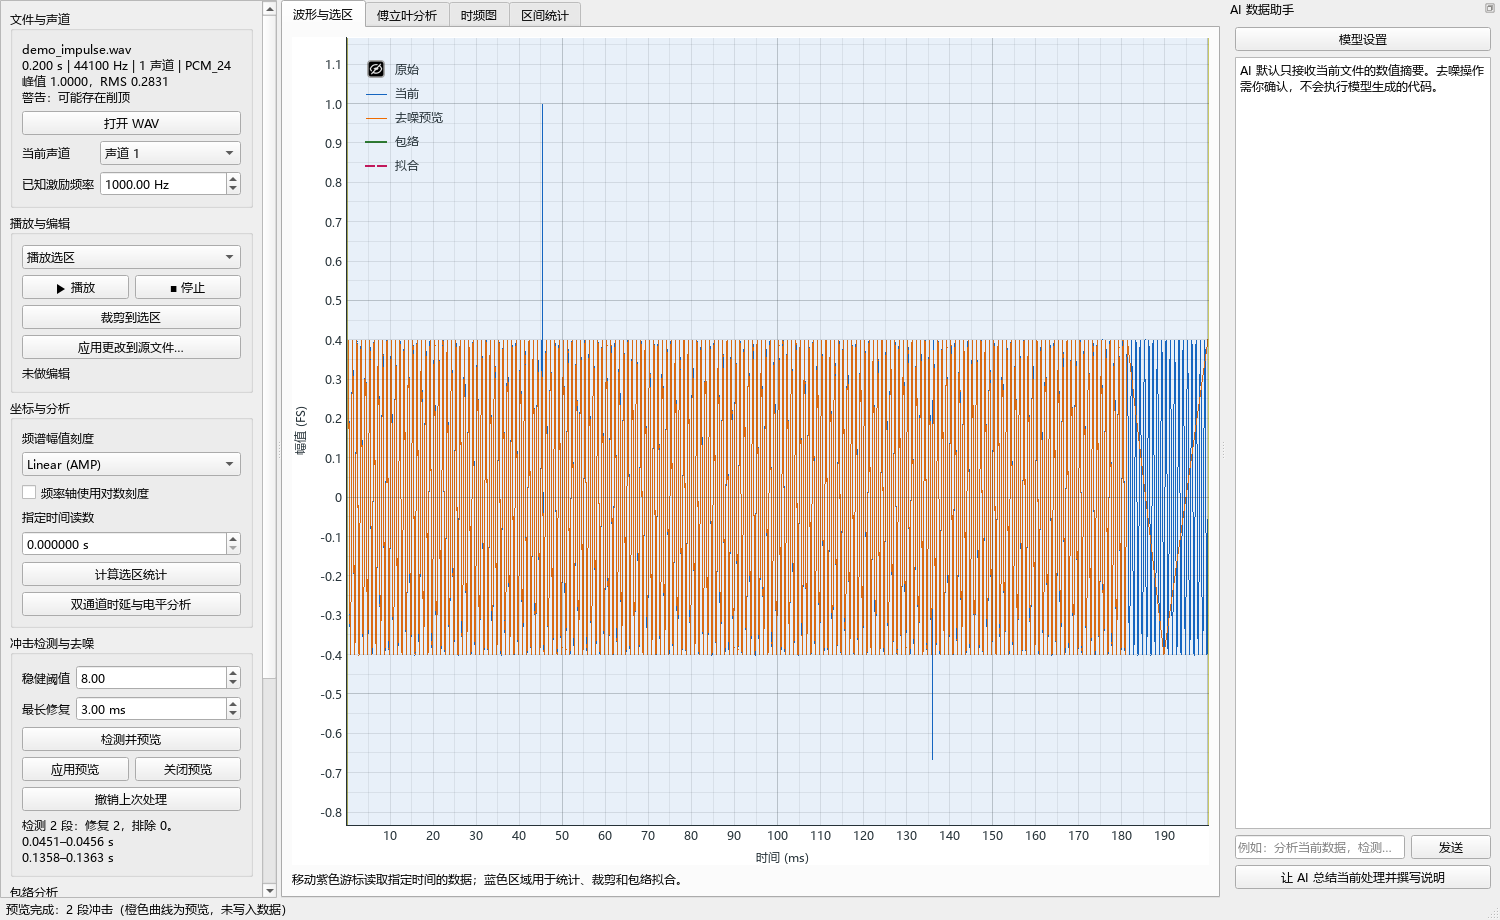
\includegraphics[width=0.96\textwidth]{01_waveform_denoise.png}
\caption{The program's main window (Waveform \& Selection tab, with a denoising preview). The left side is the control area, the center is the plot panel, and the right side is the AI data assistant.}
\label{fig:waveform}
\end{figure}

\begin{table}[htbp]
\centering
\caption{Function of the three interface regions}
\begin{tabular}{@{}>{\raggedright\arraybackslash}p{2.4cm}>{\raggedright\arraybackslash}p{11.6cm}@{}}
\toprule
Region & Main functions \\
\midrule
Left control area & Open file, select channel, set frequency, denoise, envelope, statistics, export and batch processing \\
Central plot panel & Four tabs: Waveform \& Selection, Fourier Analysis, Spectrogram, Interval Statistics \\
Right AI assistant & Model settings, session input, AI analysis and report description \\
\bottomrule
\end{tabular}
\end{table}

\subsection{Common Controls}

The left control area is grouped by function; the main controls are:

\begin{itemize}
  \item \textbf{Open WAV}: choose the recording file to analyze.
  \item \textbf{Current channel}: for two-channel files, view channel 1 and channel 2 separately; they are never mixed automatically.
  \item \textbf{Known excitation frequency}: enter the frequency actually used in the experiment; if unsure, set it to 0 and let the program estimate it.
  \item \textbf{Spectrum amplitude scale}: switch between Linear (AMP) and dBFS.
  \item \textbf{Logarithmic frequency axis}: for observing low frequencies or spectral features spanning several orders of magnitude.
  \item \textbf{Readout at a given time}: after entering a time, the purple cursor moves to that position and shows local amplitude and frequency information.
  \item \textbf{Blue selection}: drag the blue region on the waveform plot, used for interval statistics and envelope fitting.
\end{itemize}

At the top of the central plot panel are four tabs: ``Waveform \& Selection'', ``Fourier Analysis'', ``Spectrogram'', ``Interval Statistics''. Switching tabs does not change the loaded data or the analysis results.

% ==================== Chapter 4 ====================
\section{Data Import and File Management}

\subsection{Supported Formats and Loading Flow}

The program supports standard PCM WAV files, including mono and stereo; common bit depths such as 16-bit, 24-bit and 32-bit float can all be read. After clicking ``Open WAV'' and selecting a file, the program performs the following: reads the sample data, computes the quality report, initializes the processed version and the validity mask, clears the undo history, resets the AI session, and finally refreshes all plots.

After a successful load, the file-information area on the left shows the file name, duration, sample rate, channel count, sample format, peak and RMS. If the peak is detected to be near full scale, a ``Warning: possible clipping'' message is shown. Clipping means the signal has been truncated; the spectrum will contain extra harmonics, and the recording gain should be readjusted and the measurement repeated.

\subsection{Channel Selection}

For two-channel files, the ``Current channel'' dropdown offers ``Channel 1'' and ``Channel 2''. The default convention is: the left channel (channel 1) is the reference channel, and the right channel (channel 2) is the measurement channel. Switching channels only changes the data currently viewed and analyzed, and does not affect the other channel in the original file. All denoising, envelope and statistics operations act only on the processed version of the current channel.

\subsection{Read-Only Principle and the Processed Version}

The program keeps three sets of data in memory: the original samples (read-only), the processed samples (modifiable), and the validity mask (marking invalid intervals). On loading, the processed samples equal the original samples and the validity mask is all-valid. Before each denoising is applied, the program pushes the current processed samples and validity mask onto the undo stack, so you can roll back at any time. On export, the processed version is output, and by default nothing is written back to the raw WAV; when a write-back is truly needed, it goes through ``Apply changes to source file\dots'', and the program first generates a timestamped backup in the same directory. The undo stack keeps at most 4 levels, totalling about 1.2\,GB; beyond that, the earliest record is discarded.

% ==================== Chapter 5 ====================
\section{Waveform Display and Coordinate Readout}

\subsection{Elements of the Waveform Plot}

The ``Waveform \& Selection'' tab is shown in Figure~\ref{fig:waveform}; the horizontal axis is time (unit s) and the vertical axis is the digital full-scale normalized amplitude (unit FS). The curves in the waveform plot mean the following:

\begin{itemize}
  \item \textbf{Gray curve}: the original waveform. Shown only when the processed version differs from the original, for comparison.
  \item \textbf{Blue curve}: the waveform of the current processed version.
  \item \textbf{Orange curve}: the denoising-preview curve. It appears after clicking ``Detect \& preview'' and is not written into the processed version before you confirm.
  \item \textbf{Green curve}: the Hilbert envelope.
  \item \textbf{Pink dashed line}: the envelope-fit curve.
  \item \textbf{Blue translucent selection}: the interval currently used for statistics and envelope fitting.
  \item \textbf{Purple vertical line}: the time cursor.
\end{itemize}

\subsection{The Blue Selection}

The blue translucent region on the waveform plot is the current selection. By default it covers the whole file. Dragging the selection edges adjusts the start and end points. The selection is used for two operations: clicking ``Compute selection statistics'' only counts data inside the selection; clicking ``Show envelope and fit selection'' only fits the envelope model within the selection. Signals outside the selection are not used by these two operations but do fully participate in Fourier analysis and spectrogram plotting.

\subsection{Readout at a Given Time}

There are two ways to read data at a given time: drag the purple cursor directly; or enter a time value in the ``Readout at a given time'' box on the left, and the cursor moves there automatically. The readout\footnote{The readout includes the local amplitude, frequency and other information at the current time; the exact fields follow what the program displays.} is shown in the hint bar below the waveform plot. The input box supports 6 decimal places, suitable for precisely locating the instant an impulse occurs.

\subsection{Amplitude Scale and Frequency-Axis Scale}

The ``Spectrum amplitude scale'' dropdown on the left offers two choices: Linear (AMP) shows the linear amplitude of the single-sided amplitude spectrum, and dBFS shows the corresponding decibel value. dBFS is defined as $20\log_{10}(A/A_{\text{FS}})$, where $A_{\text{FS}}$ is digital full scale. Because the program applies coherent-gain correction to the window function, the spectral peak amplitude can be compared directly with the peak amplitude of the original signal.

The ``Frequency axis uses logarithmic scale'' checkbox switches the horizontal axis of the spectrum plot and the phase plot. When analyzing low-frequency phenomena or comparing frequency components across orders of magnitude, a logarithmic axis is more intuitive; when observing the distribution of high-frequency harmonics, a linear axis is clearer.

% ==================== Chapter 6 ====================
\section{Fourier Analysis}

\subsection{Basic Principle}

Fourier analysis decomposes a time-domain signal into sinusoidal components of different frequencies. The program applies a window to the entire processed version of the current channel and then performs a fast Fourier transform (FFT); the window is applied to reduce spectral leakage. The single-sided amplitude spectrum is corrected by the window's coherent gain, so the height of a spectral peak corresponds to the true peak amplitude of the sinusoidal component.

\subsection{Results Page}

The ``Fourier Analysis'' tab is shown in Figure~\ref{fig:fourier}; the upper half is the amplitude spectrum and phase spectrum, and the lower half is the dominant-peak table and the harmonic table.

\begin{figure}[htbp]
\centering
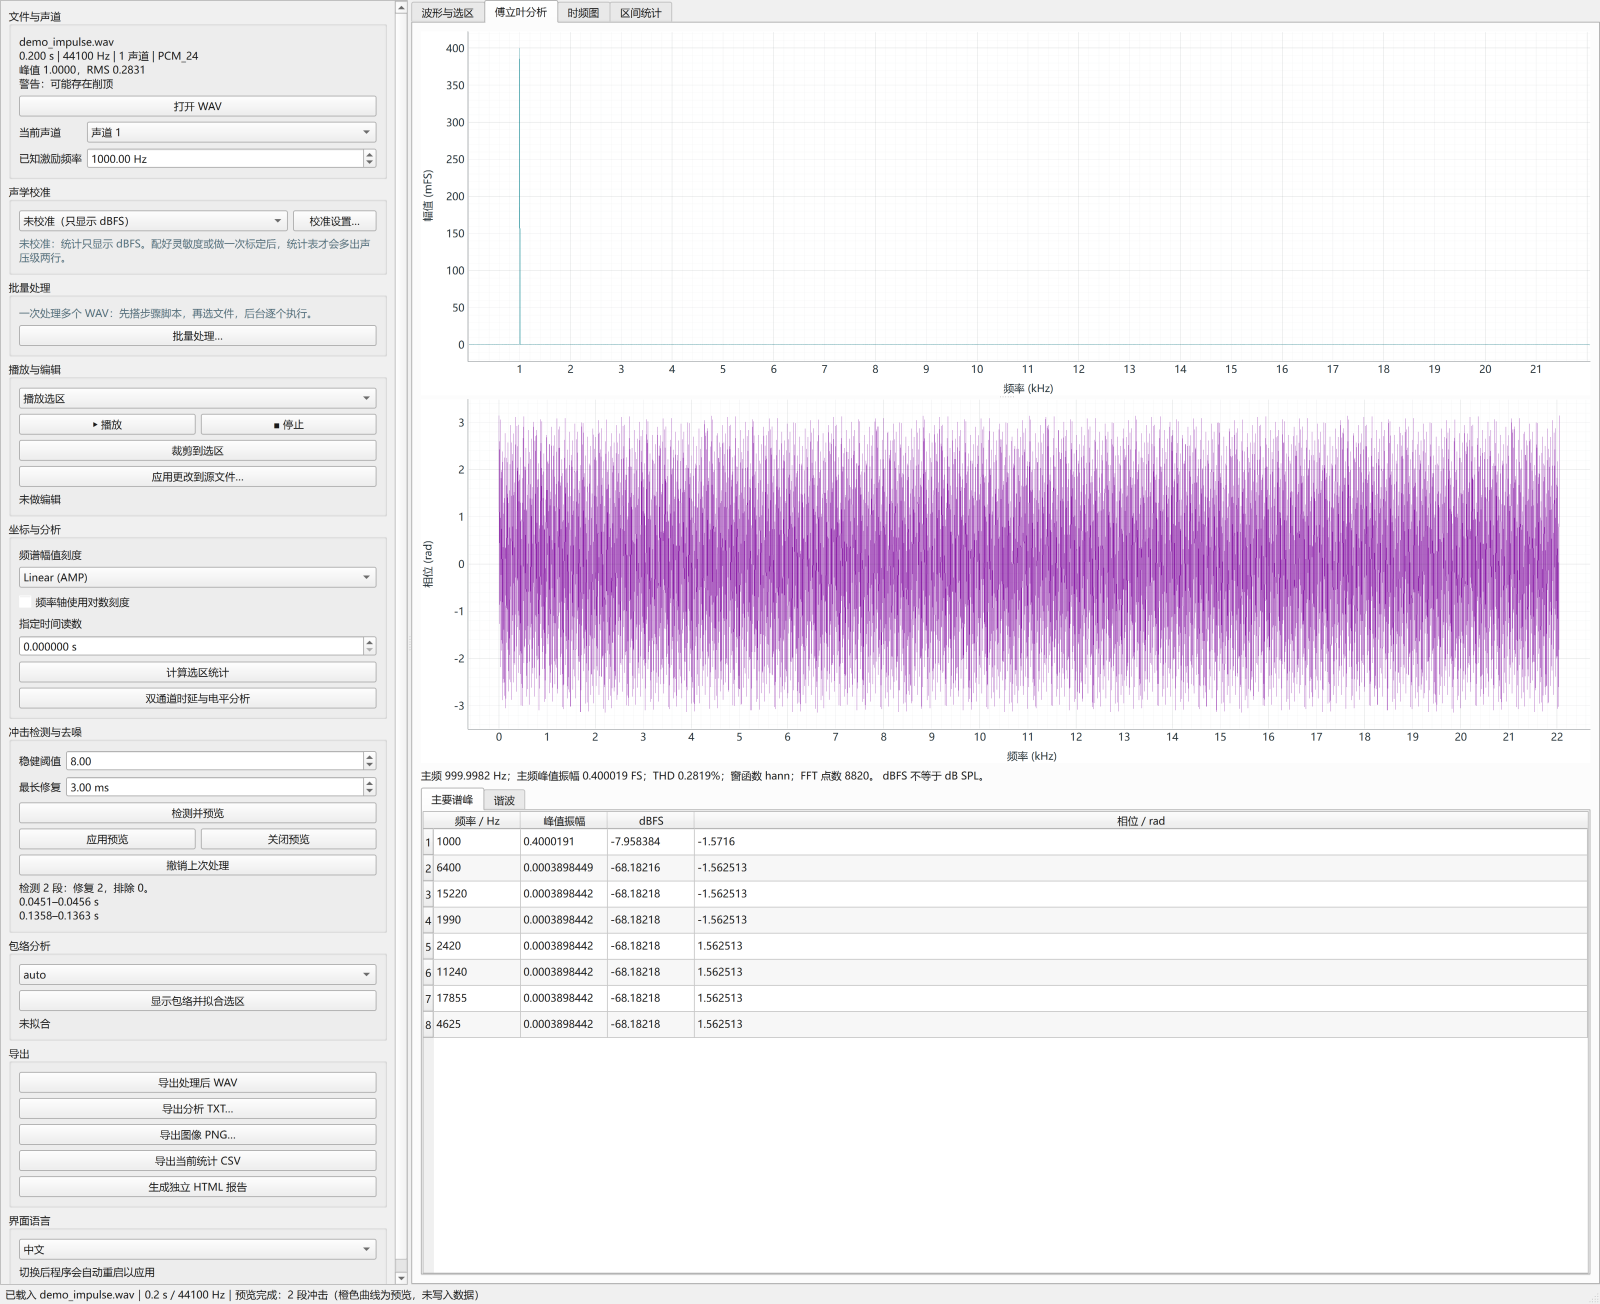
\includegraphics[width=0.96\textwidth]{02_fourier.png}
\caption{Fourier Analysis tab: top, amplitude spectrum and phase spectrum; bottom, dominant-peak table and harmonic table.}
\label{fig:fourier}
\end{figure}

The summary bar shows the following information:

\begin{itemize}
  \item \textbf{Main frequency}: the frequency component with the largest amplitude. If ``Known excitation frequency'' is set to 0, the program estimates the main frequency automatically; if set to a specific value, the program looks for a peak near that frequency.
  \item \textbf{Peak amplitude of the main frequency}: the peak amplitude corresponding to the main frequency, in FS.
  \item \textbf{THD}: total harmonic distortion, defined as the ratio of the summed energy of the harmonics to the energy of the fundamental.
  \item \textbf{Window function and FFT size}: the window type and transform size currently used.
\end{itemize}

The dominant-peak table lists the frequency, peak amplitude, dBFS and phase of significant spectral peaks. The harmonic table lists the corresponding values for harmonics 1 to 8, making it easy to observe whether the system under test introduces nonlinear distortion.

\subsection{Notes on Reading the Values}

The height of a spectral peak in the spectrum plot is affected by signal duration, window function, and frequency resolution. If the signal is too short, the frequency resolution is insufficient and adjacent spectral peaks may merge. If the signal is clipped, the spectrum will show odd-order harmonics even for a pure sine input. In that case, first check whether the waveform has flat tops, then judge whether the harmonics come from the system under test.

% ==================== Chapter 7 ====================
\section{Time--Frequency Analysis}

\subsection{Purpose of the Spectrogram}

The ``Spectrogram'' tab is shown in Figure~\ref{fig:spectrogram}; the horizontal axis is time, the vertical axis is frequency, and the color represents the energy intensity at the corresponding time and frequency. The program computes it using the short-time Fourier transform (STFT), with the viridis colormap.

\begin{figure}[htbp]
\centering
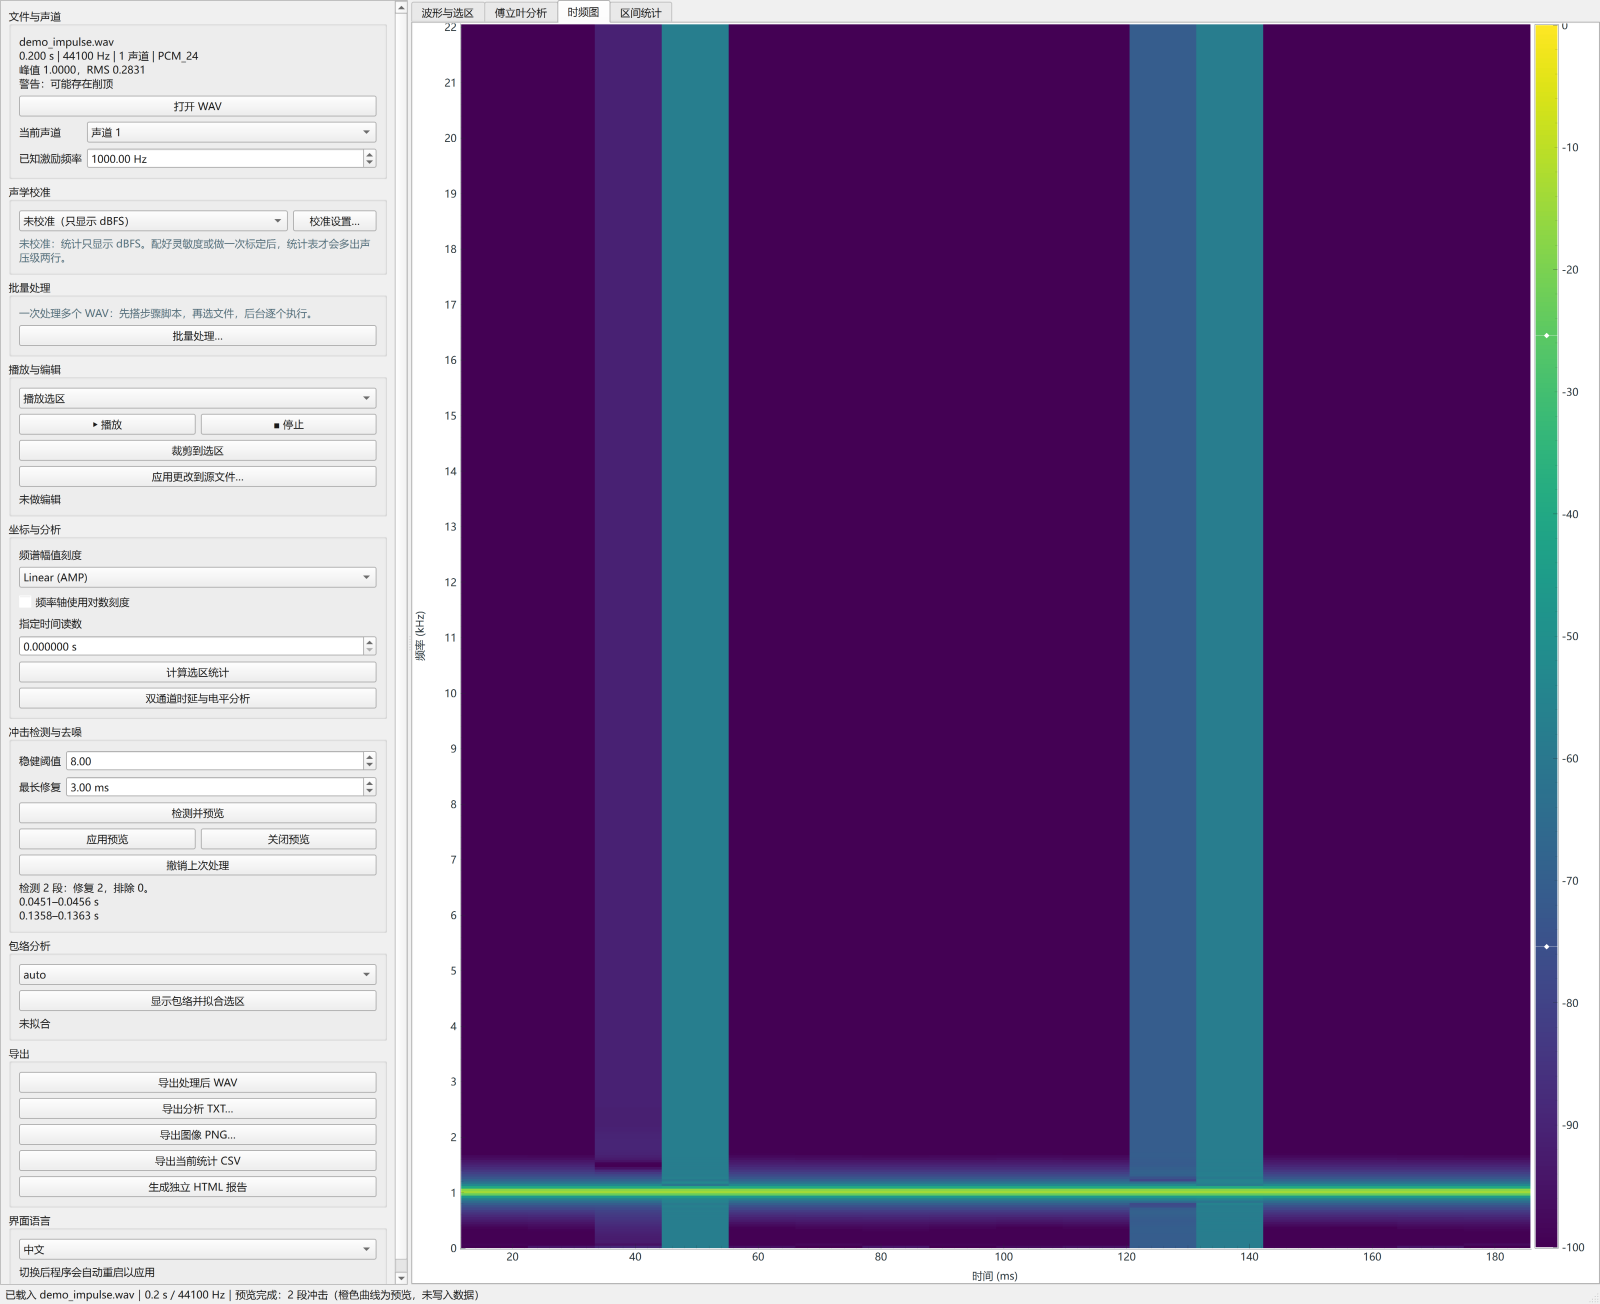
\includegraphics[width=0.96\textwidth]{03_spectrogram.png}
\caption{Spectrogram tab: a sustained sine appears as a horizontal bright band, an impulse as a short vertical wide band.}
\label{fig:spectrogram}
\end{figure}

\subsection{Reading Typical Features}

A sustained, stable sine signal appears in the spectrogram as a single horizontal bright band, whose vertical coordinate is the signal frequency. An impulse signal appears as a short, broadband vertical bright stripe spanning a wide frequency band, corresponding one-to-one with the spikes in the waveform. If there is an abrupt amplitude change (e.g., AGC kicking in), you will see the brightness of the band change suddenly in the spectrogram.

The main use of the spectrogram is to help judge whether impulse detection is reasonable: first observe the spike positions in the waveform, then confirm in the spectrogram whether they are broadband impulses, and finally compare with the repaired intervals in the denoising preview. Only when all three agree is the denoising result trustworthy.

% ==================== Chapter 8 ====================
\section{Impulse Detection and Denoising}

\subsection{Sources and Effects of Impulse Signals}

Impulse signals may come from collisions when placing the sample, sudden taps in the environment, circuit interference, or data-acquisition transients. Such signals appear as isolated spikes in the time domain and scatter energy across the whole frequency band in the frequency domain, significantly raising the high-order harmonics and the noise floor and affecting the accuracy of statistics such as RMS, crest factor and THD.

\subsection{Detection Algorithm}

The program uses robust-threshold detection: it first computes the first-order difference and the median-filter residual of the signal, then estimates a robust scale using the median absolute deviation, and finally marks samples exceeding the threshold by some multiple as impulse candidates. A robust scale is used instead of the standard deviation so that the impulses themselves do not raise the threshold and cause missed detections.

The ``Impulse detection and denoising'' group on the left provides two parameters:

\begin{itemize}
  \item \textbf{Robust threshold}: default 8.0. A larger value detects fewer events; a smaller value is more sensitive to anomalies.
  \item \textbf{Maximum repair length}: default 3.0 ms. Only impulses shorter than this length are repaired by interpolation.
\end{itemize}

\subsection{Operation Flow}

\begin{enumerate}
  \item Adjust ``Robust threshold'' and ``Maximum repair length'' on the left.
  \item Click ``Detect \& preview''.
  \item Inspect the orange preview curve and the list of event positions, comparing with the waveform plot and the spectrogram.
  \item If you judge this preview unsuitable (wrong threshold, too many false marks), click \textbf{``Close preview''} to discard it: the orange curve and the pending result are cleared together, neither the processed version nor the original file is affected, and you can change the parameters and detect again.
  \item Once satisfied, click ``Apply preview'', and only then is the preview written into the processed version.
  \item To revert, click ``Undo last processing''. Undo keeps at most the 4 most recent levels, with total usage under about 1.2 GB; beyond that, the earliest level is discarded automatically.
\end{enumerate}

The relationship among ``Detect \& preview'', ``Apply preview'' and ``Close preview'' is: \textbf{detection only produces a preview, a preview can be closed at any time, and only ``Apply preview'' changes the data.} So you can safely preview and compare with different thresholds repeatedly, without worrying about contaminating the experimental data.

\subsection{Repair and Exclusion Strategy}

The program chooses how to handle an event based on its length: impulses shorter than ``Maximum repair length'' are repaired by interpolation from surrounding samples, preserving the original waveform shape as much as possible; impulses longer than that threshold, or occurring in continuous runs, are not fabricated with signal but are marked as invalid intervals and automatically excluded from the statistical computation. This strategy avoids the algorithm ``inventing'' acoustic data that does not exist, ensuring the credibility of the experimental conclusions.

After denoising is applied, the label on the left shows the number of detected events, repairs and exclusions, and lists the start/end times of the first several event segments. The status bar shows ``Applied to the processed version; the raw WAV was not modified''.

\subsection{Points for Manual Review}

The automatic threshold has been validated on synthetic signals, but real experimental data may contain different kinds of taps, clipping and electromagnetic interference, so the automatic result must be reviewed manually. When reviewing, focus on: whether normal peaks were falsely marked, whether the impulse start and end points are accurate, and whether the excluded intervals covered valid signal. If false marks are frequent, raise the threshold, shorten the maximum repair length, and check whether the data is clipped or has a DC offset.

% ==================== Chapter 9 ====================
\section{Playback and Editing}

\subsection{Playing the Selection or the Whole File}

The ``Playback \& editing'' group on the left is for auditioning, so you do not have to switch software just to listen to a segment of the waveform.

\begin{itemize}
  \item \textbf{Playback target}: the dropdown offers ``Play selection'' or ``Play whole file''. Choosing ``Play selection'' plays only the time segment inside the blue selection.
  \item \textbf{Play and pause}: the same button toggles between ``Play'' and ``Pause''; pausing does not lose the current position.
  \item \textbf{Auto stop}: when the playback target is switched, a new file is loaded, or the window is closed, playback stops automatically and releases the audio device.
\end{itemize}

Playback only reads the processed version for monitoring; it changes no data and does not enter the undo stack. If the sound card does not support the file's sample rate (e.g., a 48\,kHz file on a device that only supports 44.1\,kHz), the program resamples automatically before playing; this resampling only affects monitoring and takes no part in any analysis, computation, or export. When no output device is available, the program shows ``There is no available audio output device on this system''; other functions are unaffected.

\subsection{Crop to Selection}

``Crop to selection'' discards the data outside the blue selection, keeping only the segment within it:

\begin{enumerate}
  \item Frame the interval you want to keep on the waveform plot. If the selection already covers the whole file, the program shows ``The current selection already covers the whole file'' and makes no change.
  \item Click ``Crop to selection''; the processed samples, validity mask, and reference waveform are cropped synchronously to the same interval.
  \item The status bar reports the kept start/end times and sample count, and the time axis is reset to zero to start afresh.
\end{enumerate}

The state before cropping is pushed onto the undo stack and can be restored at any time with ``Undo last processing''. Two common uses of cropping: first, for a long recording where you only care about one segment of response, crop first and then do statistics and envelope fitting, which greatly reduces later computation; second, crop off noisy leading/trailing segments first so that interval statistics cover only valid signal.

\subsection{Apply Changes to Source File}

By default all editing acts only on the processed version in memory, and the raw WAV stays unchanged. If you truly need to write the result back to the original file, click ``Apply changes to source file\dots'', and the program proceeds in this order:

\begin{enumerate}
  \item copies the current source file to a \texttt{.bak-timestamp.wav} backup in the same directory;
  \item writes the processed version back to the source file path in the original sample format;
  \item clears the undo stack, resets the edit count to zero, and updates the reference waveform to the written-back data.
\end{enumerate}

Write-back is not undoable: the undo stack is cleared along with it, and the only means of recovery is that backup file (rename the backup back to the original file name to restore it). The recommended order is therefore to first ``Export processed WAV'' to confirm the result is fine, then decide whether to write back to the source file. If the file is held by a player, cloud-drive sync, or antivirus, the write-back reports \texttt{PermissionError}; close the holding program and retry.

\subsection{Edit State and the Undo Stack}

The edit label shows ``N edits applied (denoise/crop), current length X s; can write back to source file or undo (K levels undoable)'', so you can always confirm how many times the current data has been changed and how many steps you can still go back. The undo stack keeps at most 4 levels, totalling about 1.2\,GB; when editing a large file repeatedly, the earliest records are discarded automatically to avoid exhausting memory. When you need to keep an intermediate result for a long time, export the processed WAV rather than relying on the undo stack.

% ==================== Chapter 10 ====================
\section{Envelope Analysis}

\subsection{Principle of Envelope Extraction}

The program uses the Hilbert transform to extract the analytic signal, whose magnitude is the instantaneous-amplitude envelope. The envelope reflects how the signal's amplitude changes over time and is suitable for analyzing decay processes, onset processes, and amplitude-modulation phenomena.

\subsection{Operation Flow and Model Selection}

First frame the interval to be analyzed on the waveform plot, then click ``Show envelope and fit selection''. The ``Envelope analysis'' group on the left provides four models:

\begin{itemize}
  \item \texttt{auto}: automatic selection; the program picks among the candidate models based on goodness of fit.
  \item \texttt{constant}: constant model, suitable for steady signals.
  \item \texttt{linear}: linear model, suitable for slowly rising or falling amplitude changes.
  \item \texttt{exponential}: exponential model, suitable for decay processes.
\end{itemize}

\begin{figure}[htbp]
\centering
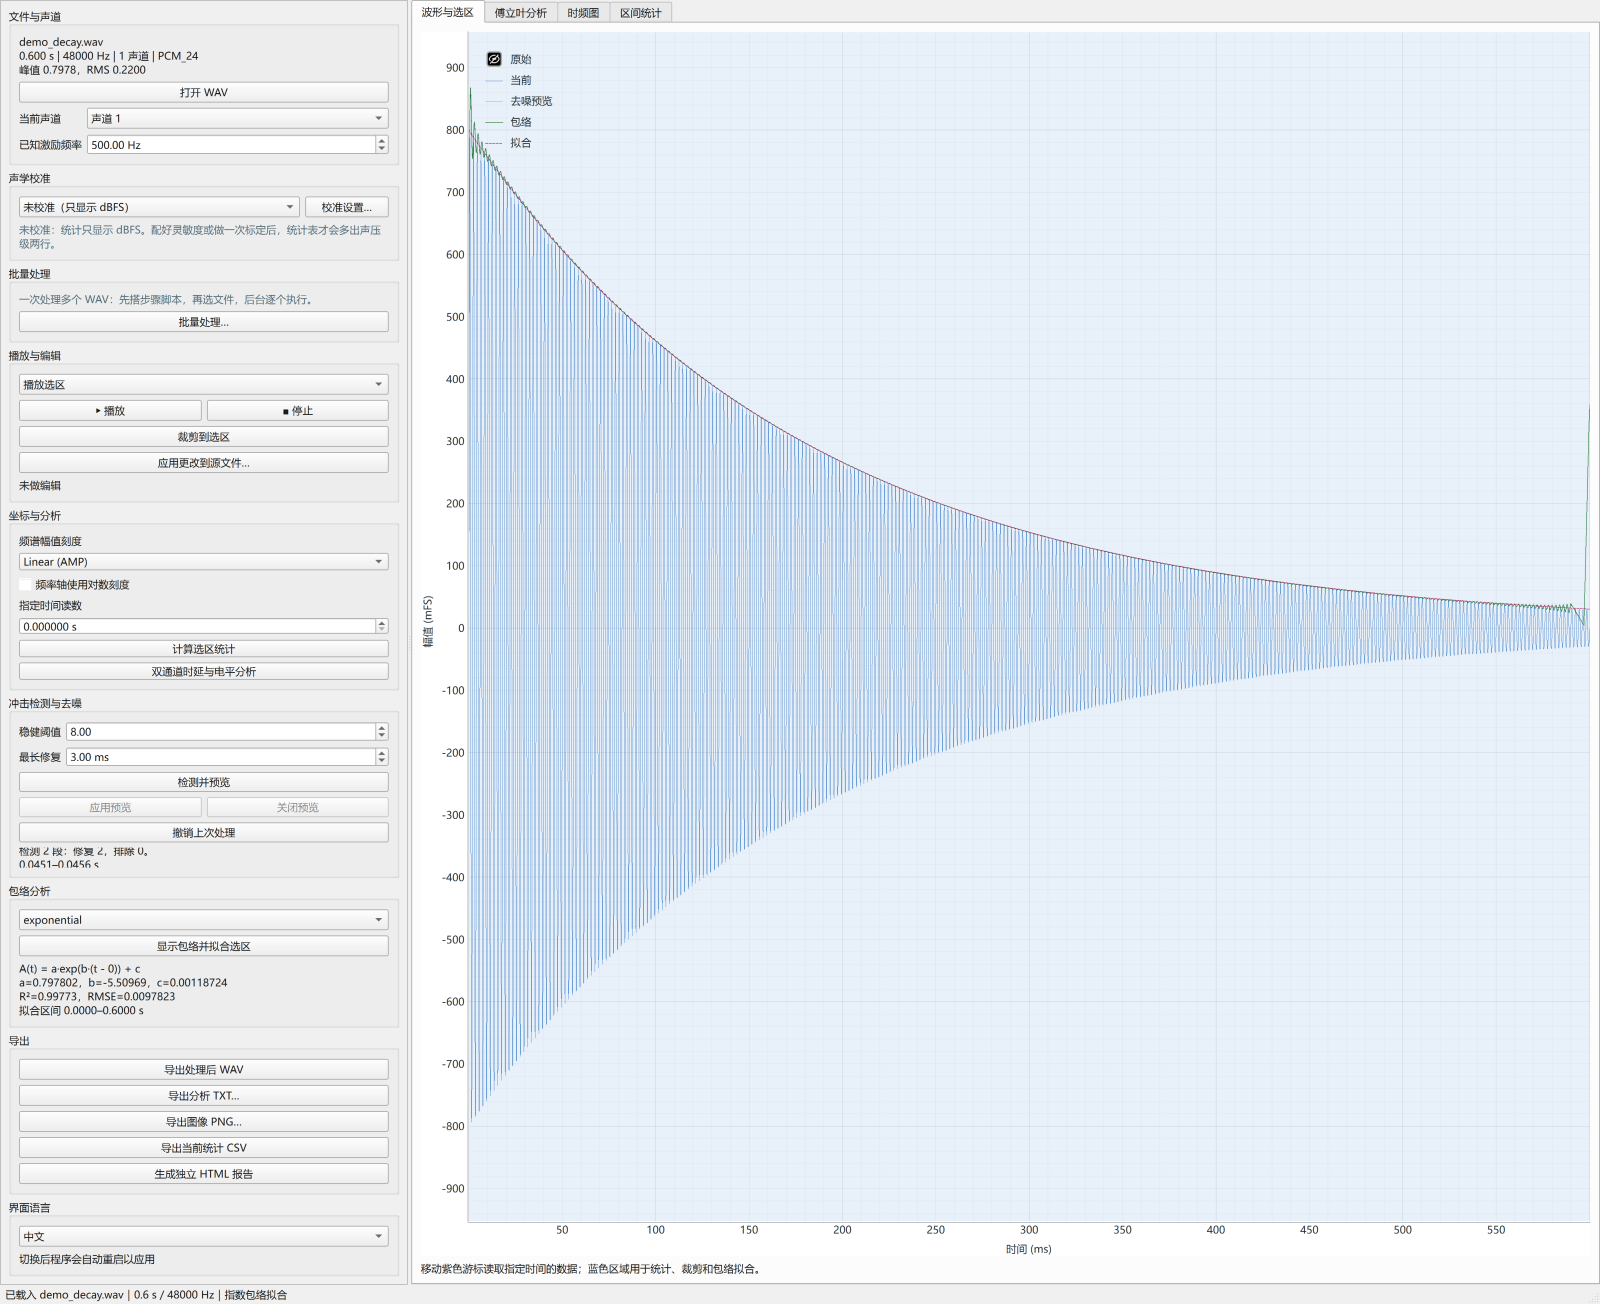
\includegraphics[width=0.96\textwidth]{05_envelope.png}
\caption{Envelope analysis: green is the Hilbert envelope, the pink dashed line is the fit curve within the selection.}
\label{fig:envelope}
\end{figure}

As shown in Figure~\ref{fig:envelope}, the fit result includes the envelope equation, the parameter values, the coefficient of determination $R^2$, and the root-mean-square error RMSE. A steady sine usually approaches a constant envelope; for a decay process you can try the exponential model. If $R^2$ is very low or the residuals are anomalous, check whether the selection includes onset/offset transients, impulses, or AGC changes.

% ==================== Chapter 11 ====================
\section{Interval Statistics}

\subsection{Description of the Statistics}

The ``Interval Statistics'' tab is shown in Figure~\ref{fig:statistics}. After clicking ``Compute selection statistics'', the program computes the following statistics within the current blue selection:

\begin{figure}[htbp]
\centering
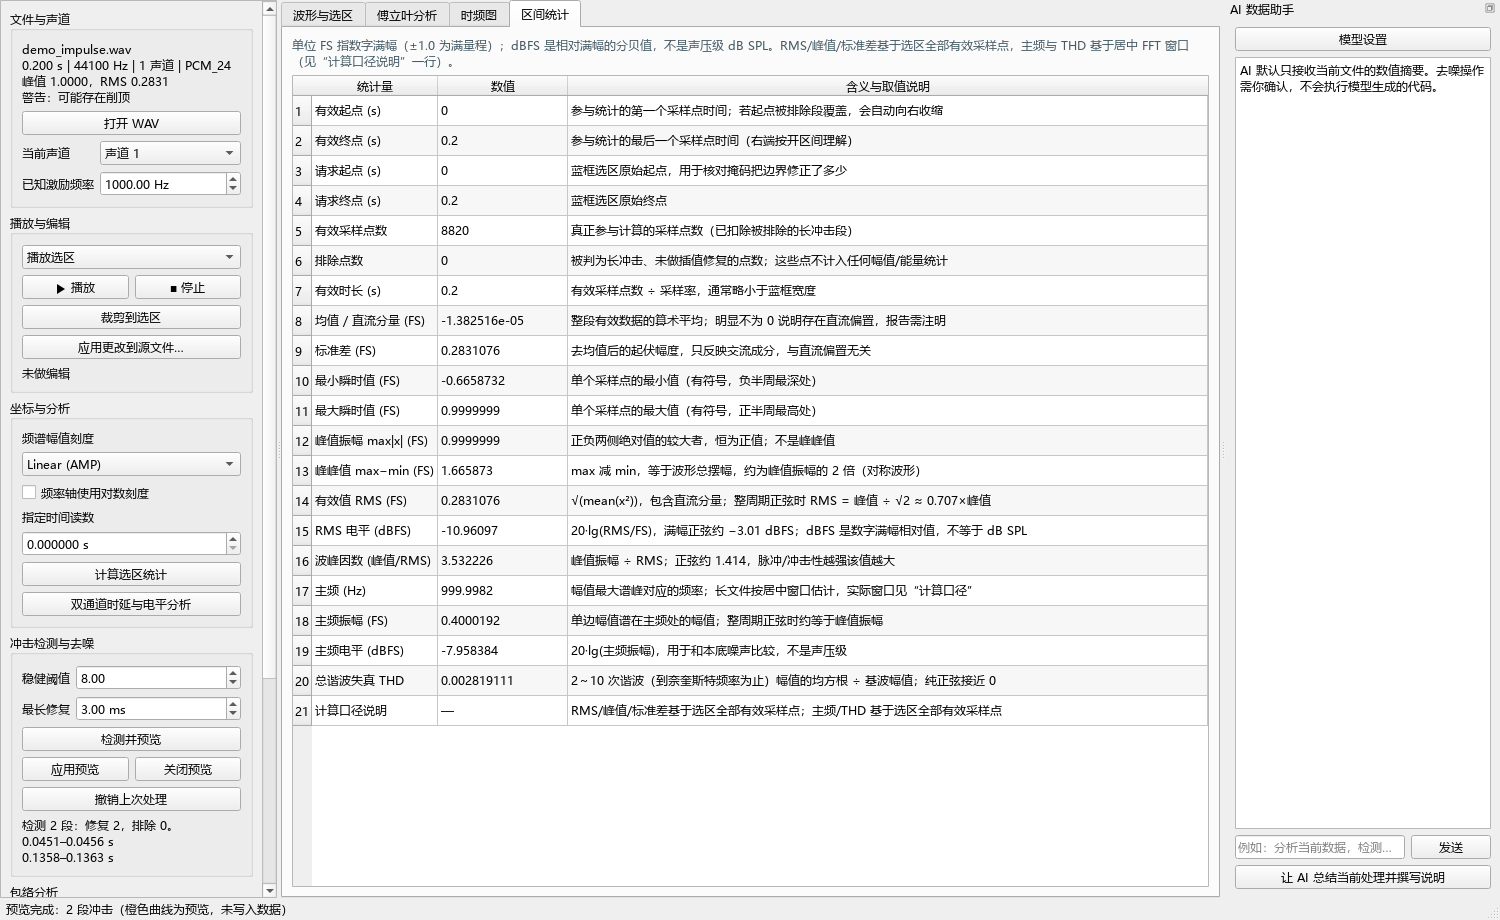
\includegraphics[width=0.96\textwidth]{04_statistics.png}
\caption{Interval Statistics tab: displays the statistics within the selection in table form.}
\label{fig:statistics}
\end{figure}

The program's statistics table uses three columns: \textbf{statistic (name)}, \textbf{value}, and \textbf{meaning and value notes}. Only the quantities whose names alone are easily confused (for example ``peak amplitude'' vs.\ ``peak-to-peak'', ``RMS'' vs.\ ``RMS level'') have their differences spelled out in the third column; the table below corresponds row by row to the program interface.

{\small
\begin{longtable}{@{}p{0.22\textwidth}p{0.26\textwidth}p{0.44\textwidth}@{}}
\caption{Interval statistics glossary (one-to-one with the program's ``Interval Statistics'' tab)}\\
\toprule
Displayed name & Key & Meaning and value notes \\
\midrule
\endfirsthead
\toprule
Displayed name & Key & Meaning and value notes \\
\midrule
\endhead
\bottomrule
\endfoot
Valid start (s) & \texttt{start\_s} & time of the first sample included in the statistics; if the start is covered by an excluded segment, it automatically shrinks to the right \\
Valid end (s) & \texttt{end\_s} & time of the last sample included in the statistics (understand the right end as an open interval) \\
Requested start (s) & \texttt{requested\_start\_s} & the original start of the blue selection, used to check how much the mask moved the boundary \\
Requested end (s) & \texttt{requested\_end\_s} & the original end of the blue selection \\
Valid samples & \texttt{samples} & the number of samples actually used in the computation, with excluded long-impulse segments already subtracted \\
Excluded samples & \texttt{excluded\_samples} & the number of points judged as long impulses and not repaired by interpolation; they enter no amplitude or energy statistic \\
Valid duration (s) & \texttt{duration\_s} & valid samples $\div$ sample rate, usually slightly smaller than the width of the blue selection \\
Mean / DC offset (FS) & \texttt{mean} & the arithmetic mean of the valid data; clearly nonzero indicates a DC offset, which the report should note \\
Std.\ deviation (FS) & \texttt{std} & the fluctuation magnitude after removing the mean; reflects only the AC component and is unrelated to the DC offset \\
Min instantaneous (FS) & \texttt{min} & the minimum of a single sample (signed, the deepest point of the negative half-cycle) \\
Max instantaneous (FS) & \texttt{max} & the maximum of a single sample (signed, the highest point of the positive half-cycle) \\
Peak amplitude (FS) & \texttt{peak\_amplitude} & $\max|x|$, always positive; not peak-to-peak, and not RMS \\
Peak-to-peak (FS) & \texttt{peak\_to\_peak} & $\max-\min$, the total swing of the waveform; for a symmetric waveform it is about twice the peak amplitude \\
RMS (FS) & \texttt{rms} & the root mean square $\sqrt{\mathrm{mean}(x^2)}$, including the DC component; for a whole-period sine it equals peak $\div$ $\sqrt{2}$ \\
RMS level (dBFS) & \texttt{rms\_dbfs} & $20\lg(\mathrm{RMS}/\mathrm{FS})$, a full-scale sine is about $-3.01$ dBFS; dBFS is not the sound pressure level dB SPL \\
Crest factor & \texttt{crest\_factor} & peak amplitude $\div$ RMS; a sine is about 1.414, and the more impulsive/pulsed the signal, the larger this value \\
Main frequency (Hz) & \texttt{main\_frequency\_hz} & the frequency of the largest-amplitude spectral peak; for long files it is estimated on a centered window, the actual window is given in ``Analysis scope'' \\
Main amplitude (FS) & \texttt{main\_amplitude} & the single-sided amplitude spectrum's value at the main frequency; for a whole-period sine it is about equal to the peak amplitude \\
Main level (dBFS) & \texttt{main\_amplitude\_dbfs} & $20\lg(\text{main amplitude})$, used for comparison with the noise floor; not a sound pressure level \\
THD & \texttt{thd} & the root mean square of harmonics 2--10 (up to the Nyquist frequency) divided by the fundamental amplitude; a pure sine is close to 0 \\
Analysis scope & \texttt{analysis\_scope} & states which quantities are based on all samples of the selection and which are based on a limited FFT window \\
\end{longtable}
}

When exporting CSV, the key names in the second column are used, which makes batch processing by scripts easy; the interface, the HTML report, and the AI description use the displayed names. Both refer to the same quantity.

\subsection{Handling of Invalid Intervals}

The statistics automatically exclude long-impulse intervals already marked invalid. This means that even if the selection covers the whole recording, samples in the excluded intervals do not enter the computation. If you need to statistics a particular steady segment, it is recommended to shrink the blue selection manually to avoid the influence of onset/offset transients.

The results can be saved as a CSV file via the ``Export current statistics CSV'' button on the left, for further processing in Excel or Python.

\subsection{Long-Audio Processing and Numerical Conventions}

The experimental recordings this program targets may be very long (for example, over ten minutes, tens of millions of samples). To keep the interface responsive when analyzing extremely long files, the program optimizes display and spectral computation. Understanding the computation convention for each kind of data is crucial to citing experimental results correctly:

\begin{itemize}
  \item \textbf{Energy-type statistics} (RMS, peak, peak-to-peak, mean, standard deviation, crest factor): always computed from the \textbf{full set of valid samples} in the selected interval, with no decimation, so accuracy is unaffected.
  \item \textbf{Main frequency and THD}: to avoid the long stalls of a full-length FFT, these are by default computed on a centered window of about 5.5 seconds (262{,}144 points), with frequency resolution about \texttt{sample\_rate/262144} (about 0.18 Hz at 48 kHz). The ``Fourier Analysis'' tab and the status bar explicitly label the actual analyzed time range and point count; the program never silently analyzes only local data. If you need higher frequency resolution (e.g., precise steady-state calibration), you can call \texttt{fourier\_analysis(..., max\_samples=0)} in the source for a full-length analysis.
  \item \textbf{Waveform display and spectrogram}: only visualization decimation is done (the waveform keeps per-column extrema, the spectrogram skips frames); these \textbf{take no part in any numerical computation} and therefore do not affect the statistics. The spectrogram's time sampling is sparse, so for short impulses it is recommended to use the waveform plot as the primary locator.
  \item \textbf{Cursor envelope readout}: uses a centrally symmetric window to compute the Hilbert envelope and takes the center value, avoiding edge effects from introducing systematic bias on steady signals.
\end{itemize}

When citing spectral quantities such as main frequency and THD in an experimental report, also record the analysis window and point count labeled by the program, so the result can be reproduced.

% ==================== Chapter 12 ====================
\section{Acoustic Calibration}

\subsection{Why Calibration Is Needed}

Every amplitude inside the program is relative to digital full scale: FS denotes the ratio of $|x|$ to full scale, and dBFS is $20\lg|x|$. For comparing two segments within the same recording, this relative unit is entirely sufficient; but an experimental report often needs an absolute sound pressure level, which requires anchoring the reading to a specific microphone.

The conversion needs only a single additive constant. Let the microphone sensitivity be $S$ (V/Pa), the preamplifier gain $G$ (a linear factor, $G=10^{G_\mathrm{dB}/20}$), and the input voltage corresponding to 0\,dBFS on the sound card $V_\mathrm{fs}$; then

\begin{equation}
L_\mathrm{SPL} = L_\mathrm{dBFS} + K, \qquad
K = 20\lg\frac{V_\mathrm{fs}}{G\,S\,p_0}, \qquad p_0 = 20\ \mu\mathrm{Pa}.
\label{eq:calib}
\end{equation}

The derivation has only three steps: input voltage $V_\mathrm{adc} = V_\mathrm{fs}\cdot10^{L_\mathrm{dBFS}/20}$, sound pressure $p = V_\mathrm{adc}/(GS)$, then take 20 times the logarithm of $p/p_0$. All three steps are multiplication/division, which become addition/subtraction after taking the logarithm, so a whole batch of data shares the same $K$---calibrate once, and every row after that is a simple addition.

Taking a common electret capsule as an example: with $S=10$\,mV/Pa, no preamplifier gain, and a sound-card full scale of 1\,Vrms, we get $K=+133.98$\,dB. Check: 94\,dB SPL corresponds exactly to 1\,Pa, the microphone outputs 10\,mV, which relative to 1\,Vrms is $-40$\,dBFS, and $-40+133.98=93.98$, differing from the nominal value by only 0.02\,dB (due to rounding).

\subsection{Two Input Methods}

In the ``Acoustic calibration'' group on the left, click ``Calibration settings\dots'' to open the dialog in Figure~\ref{fig:calib_params}. There are two ways to obtain $K$, and they are equivalent:

\begin{figure}[H]
\centering
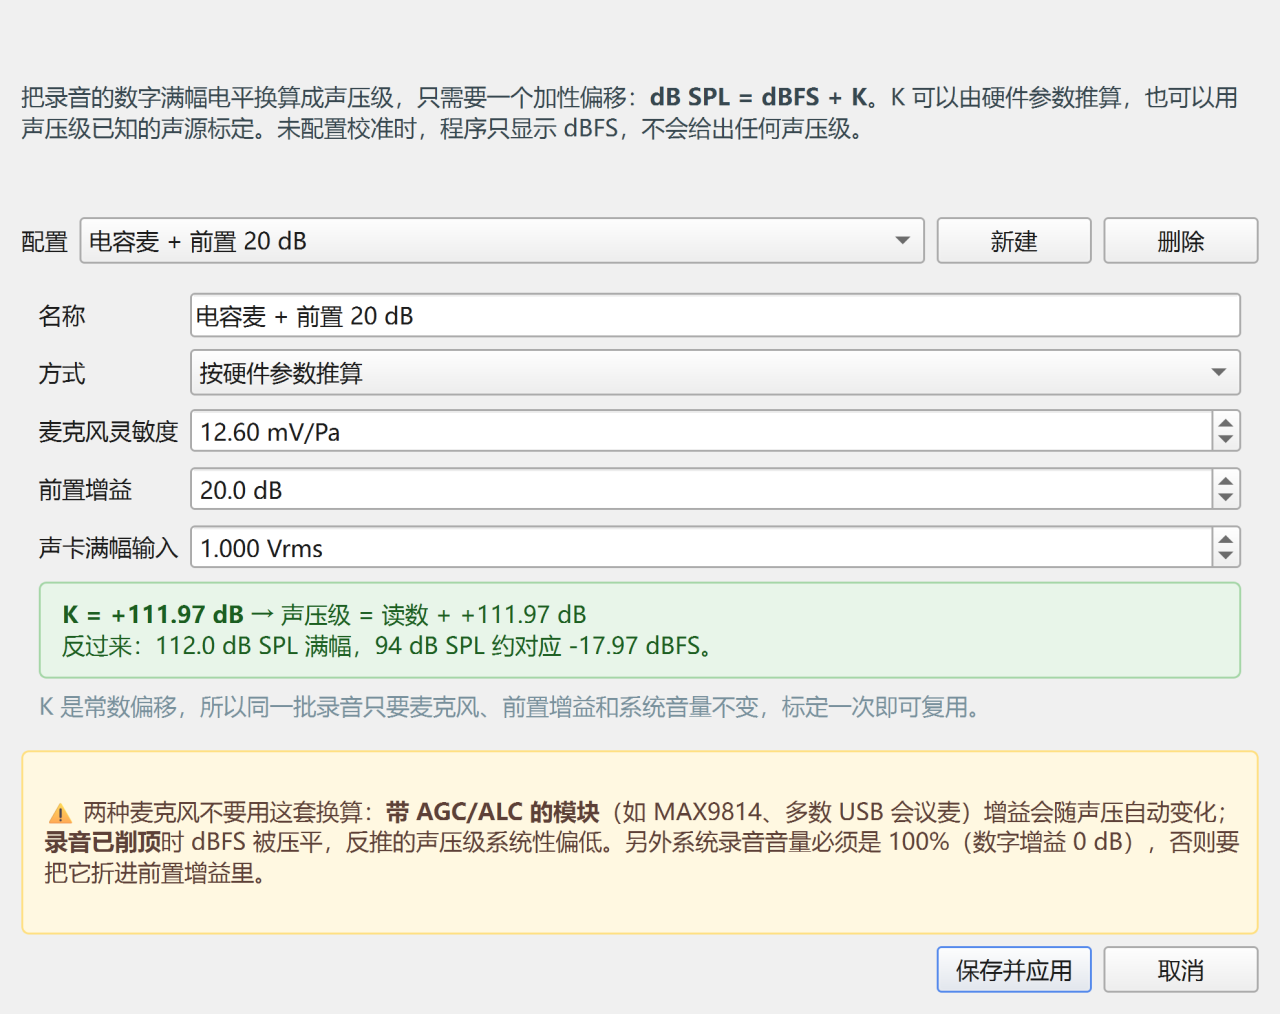
\includegraphics[width=0.84\textwidth]{13_calibration.png}
\caption{Compute from hardware parameters. The green box gives $K$ in real time and back-calculates ``about what dBFS corresponds to 94 dB SPL'', convenient for an on-the-spot check.}
\label{fig:calib_params}
\end{figure}

\begin{itemize}
  \item \textbf{Compute from hardware parameters}: fill in sensitivity, preamplifier gain, and the sound card's full-scale input voltage. Table~\ref{tab:calib_examples} gives $K$ for several common chains, useful for checking whether the parameters you entered are reasonable.
  \item \textbf{Calibrate with a known sound pressure level}: take a source with a known sound pressure level (a sound-level calibrator, or a calibrated phone playing a fixed tone), enter its nominal SPL and the dBFS read by the program, and $K=L_\mathrm{ref}-L_\mathrm{dBFS}$. This route does not require knowing $V_\mathrm{fs}$---and $V_\mathrm{fs}$ is precisely the least reliable parameter of a consumer sound card.
\end{itemize}

\begin{table}[htbp]
\centering
\caption{Calibration offsets for several common chains ($V_\mathrm{fs}$ taken as the nominal value; the actual value may differ)}
{\small
\begin{tabular}{@{}>{\raggedright\arraybackslash}p{3.0cm}>{\raggedright\arraybackslash}p{2.4cm}>{\raggedright\arraybackslash}p{2.4cm}>{\raggedright\arraybackslash}p{1.9cm}>{\raggedright\arraybackslash}p{4.4cm}@{}}
\toprule
Chain & Sensitivity & Preamp gain & $K$ / dB & Note \\
\midrule
Electret + sound card & 10 mV/Pa & 0 dB, 1 Vrms & 133.98 & textbook baseline \\
As above + preamp & 10 mV/Pa & 20 dB, 1 Vrms & 113.98 & for every 20 dB more gain, $K$ drops 20 \\
High-sensitivity condenser mic & 50 mV/Pa & 0 dB, 1 Vrms & 120.00 & 14 dB more sensitive, 14 lower $K$ \\
Pro audio interface & 12.6 mV/Pa & 20 dB, 0.775 Vrms & 109.76 & full scale taken as $-2.2$ dB, $K$ a bit lower \\
\bottomrule
\end{tabular}}
\label{tab:calib_examples}
\end{table}

The second image is the calibration-by-reference method (Figure~\ref{fig:calib_ref}). Clicking ``Take current statistics'' fills the current selection's RMS level directly into ``corresponding reading'', sparing you manual copying; the prerequisite is that selection statistics have been computed once.

\begin{figure}[H]
\centering
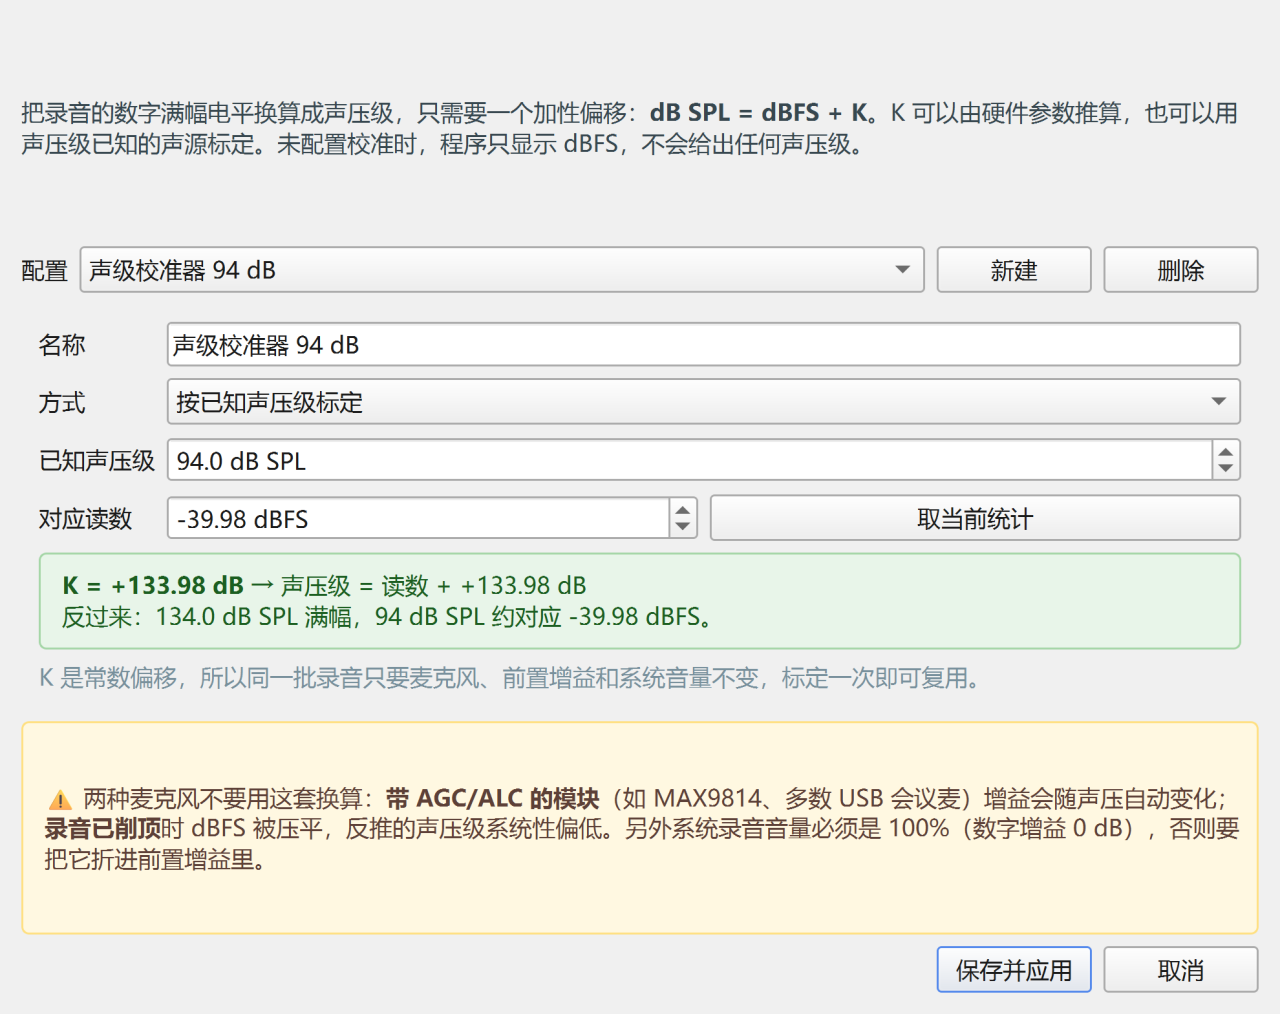
\includegraphics[width=0.84\textwidth]{14_calibration_ref.png}
\caption{Calibrate with a known sound pressure level. Parameters such as sensitivity and gain are hidden here, leaving only the two rows ``known SPL'' and ``corresponding reading''.}
\label{fig:calib_ref}
\end{figure}

\begin{quote}
\textbf{The correct way to calibrate}: set the source steadily to its nominal SPL (for example, mount the calibrator on the microphone at 94 dB SPL) and record for more than 3 seconds; in the program select this steady interval, click ``Compute selection statistics'', and read the RMS level; then in the calibration dialog choose ``Calibrate with a known SPL'' and click ``Take current statistics''. The accuracy of this route depends on whether the source itself is trustworthy, not on the sound card's parameters.
\end{quote}

\subsection{How Calibration Affects the Results}

The calibration configuration is stored locally (in the same configuration store as the AI settings), can be saved multiple times, and is switched by name. When switching configurations, \textbf{already-computed statistics have their sound pressure levels recomputed in place}, without redoing the FFT---the statistics themselves have not changed, only an additive offset has, so switching is instantaneous.

The changes to several outputs are listed in Table~\ref{tab:calib_outputs}.

\begin{table}[htbp]
\centering
\caption{What changes in each place after configuring calibration}
{\small
\begin{tabular}{@{}>{\raggedright\arraybackslash}p{3.4cm}>{\raggedright\arraybackslash}p{10.4cm}@{}}
\toprule
Location & Change \\
\midrule
Interval statistics table & two new rows ``peak SPL'' and ``equivalent SPL'', placed right after the corresponding dBFS rows; the last two rows give $K$ and the configuration name \\
Statistics CSV & three extra columns \texttt{peak\_spl}, \texttt{rms\_spl}, \texttt{calibration\_offset\_db}; the dBFS columns are still kept \\
Analysis TXT & a ``Acoustic calibration'' line (configuration name and $K$) is added to the file header, followed by three qualifying lines; the interval-statistics section gains two rows in sync \\
HTML report & the statistics table gains two rows in sync, the footer note changes to ``converted by acoustic calibration'', and it notes that no frequency weighting is applied \\
Batch processing & the whole batch shares the calibration group currently selected in the main window; the merged CSV and TXT outputs also carry SPL \\
\bottomrule
\end{tabular}}
\label{tab:calib_outputs}
\end{table}

\textbf{When no calibration is configured, the program outputs no dB SPL field at all.} This is intentional: filling in a plausible-looking number that has no calibration basis is far more dangerous than leaving it blank.

\needspace{9\baselineskip}
\subsection{When This Conversion Does Not Hold}

\begin{enumerate}
  \item \textbf{Microphones with AGC/ALC} (MAX9814 modules, most USB conference mics): the gain changes automatically with sound pressure, so $K$ is not a constant. Such devices can only do relative comparison, not give absolute SPL.
  \item \textbf{Recording already clipped}: after clipping, dBFS is flattened near 0, and the back-calculated SPL is systematically low. First look at the clipping warning in the quality check.
  \item \textbf{System recording volume not at 100\%}: Windows' input volume is a digital gain, equivalent to adding a term to $G$. Either fix it at 100\%, or fold that term into the ``preamplifier gain'' field.
  \item \textbf{Sound-card full-scale voltage unknown or nominal value inaccurate}: this is the largest source of uncertainty in the parameter-computation route. If conditions allow, switch to calibration by a known SPL.
  \item \textbf{A quantity that needs frequency weighting}: the program gives the unweighted (Z-weighted) sound pressure level, not dBA. To report dBA, weight in the frequency domain by the A-weighting curve and then integrate.
\end{enumerate}

\subsection{A Complete Calibration Example}

Take a typical transmission-measurement chain ``electret microphone $\to$ 30 dB preamplifier $\to$ USB sound card (full scale 1 Vrms)'', with the microphone's nominal sensitivity 12.6 mV/Pa:

\begin{enumerate}
  \item Compute $K$: $K = 133.98 - 20\lg(12.6/10) - 30 = 133.98 - 2.01 - 30 = 101.97$\,dB.
  \item Enter $S=12.6$, gain 30, full scale 1.0 in the dialog, and confirm the green box shows $K=+101.97$\,dB.
  \item Save it as ``Electret +30 dB''; thereafter it is reused automatically each time you open the program.
  \item Record a known source (e.g., a 94 dB calibrator) to verify: if the program reads $-8.03$\,dBFS, then $-8.03+101.97=93.94$, differing from the nominal value by 0.06\,dB, which shows the parameters are correct. If it differs a lot, switch to the calibration-by-reference method and set $K$ directly from the measured value.
  \item When batch-processing hundreds of files, this selected calibration group takes effect for the whole batch; the CSV directly yields each measurement point's equivalent SPL and peak SPL, and subtracting to get $\Delta L$ then gives the level difference between two conditions.
\end{enumerate}

\begin{quote}
\textbf{Reminder}: $\Delta L$ is the subtraction of two SPLs, and $K$ cancels in the subtraction. So as long as the whole batch uses the same hardware and gain, even a 1\,dB bias in $K$ leaves the level difference accurate. What calibration really affects is the \textbf{absolute sound pressure level}, and whether data across different gain batches can be compared directly.
\end{quote}

% ==================== Chapter 13 ====================
\section{Dual-Channel Analysis}

\subsection{What Is Analyzed}

For a two-channel file, clicking ``Dual-channel delay and level analysis'' pops up a result window showing:

\begin{itemize}
  \item \textbf{Cross-correlation delay}: estimates the time difference between the two signals via the peak position of the cross-correlation function.
  \item \textbf{Peak quality}: the sharpness of the cross-correlation peak, reflecting the confidence of the estimate.
  \item \textbf{RMS levels of both channels}: the root-mean-square levels of channel 1 and channel 2.
  \item \textbf{Level difference}: the difference between the two levels, often used to compare the sound-level difference between two conditions.
\end{itemize}

\subsection{AGC Risk Warning}

If the recording device uses a microphone module with automatic gain control (AGC), such as the MAX9814, the microphone gain adjusts automatically with sound pressure, and the two channels' amplitude ratio no longer accurately reflects the true sound-pressure ratio. In that case the level difference cannot be taken directly as a conclusion. Strength conclusions should be combined with a sound-level-meter reading or reliable amplitude calibration, and the report must state whether AGC was active.

% ==================== Chapter 14 ====================
\section{AI Data Assistant}

\subsection{Model Configuration}

Click ``Model settings'' on the right (Figure~\ref{fig:ai_settings}). At the top of the dialog are \textbf{vendor presets}; after choosing a vendor, the Base URL and common model names are filled in automatically, and you only need to enter the API Key:

\begin{itemize}
  \item \textbf{DeepSeek}: \texttt{https://api.deepseek.com/v1}, models \texttt{deepseek-chat}, \texttt{deepseek-reasoner}.
  \item \textbf{Moonshot (Kimi)}: \texttt{https://api.moonshot.cn/v1}, models \texttt{kimi-latest}, \texttt{kimi-k2-0905-preview}, etc.
  \item \textbf{OpenAI}: \texttt{https://api.openai.com/v1}, models \texttt{gpt-4.1-mini}, etc.
  \item \textbf{Custom (fill in Base URL and model name yourself)}: for a school or lab self-hosted gateway, a proxy service, or a compatible service other than the three above; all three fields must be filled in by you.
\end{itemize}

\begin{figure}[H]
\centering
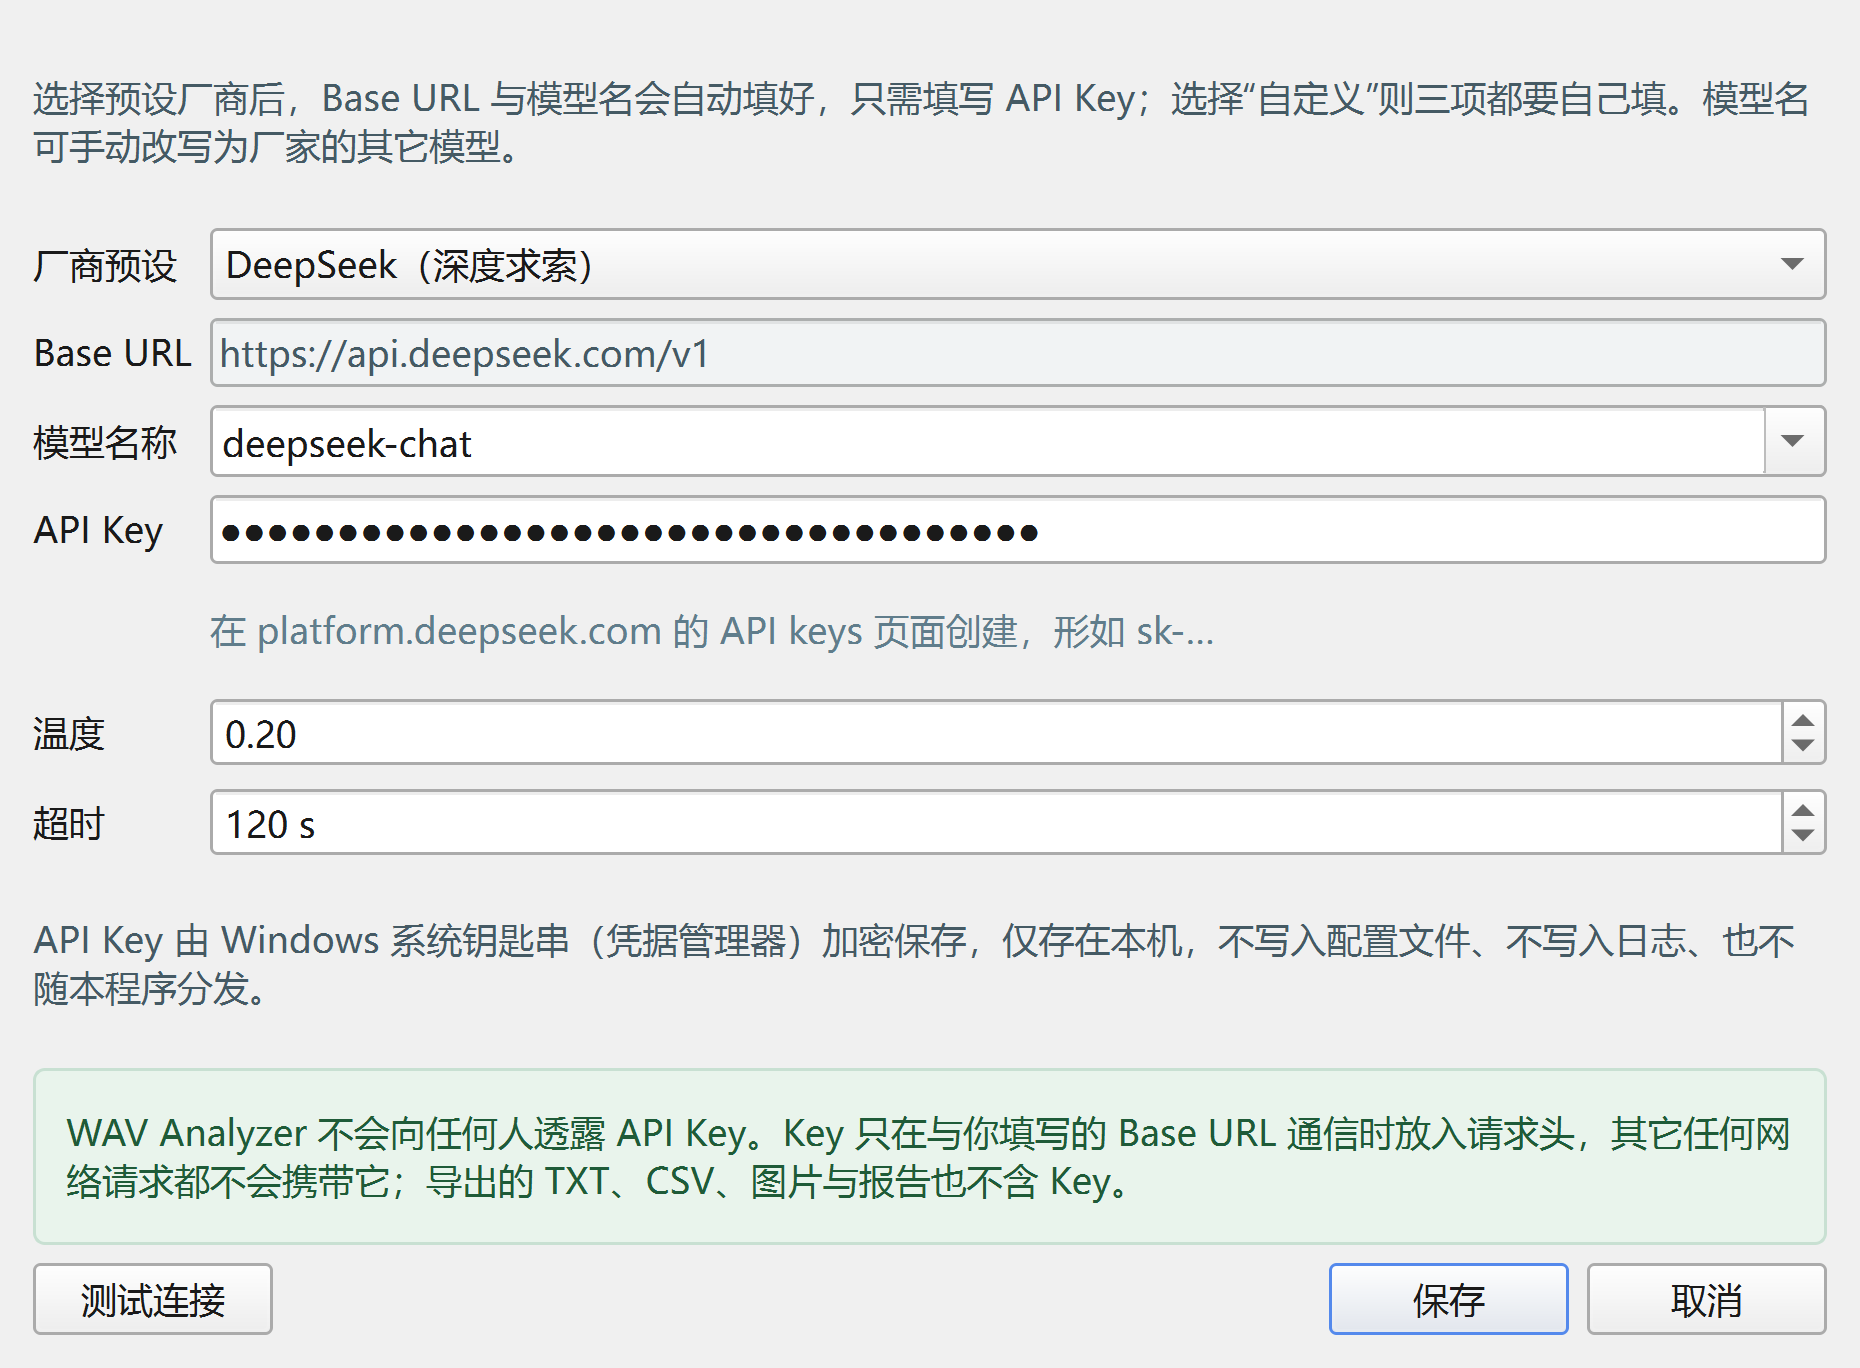
\includegraphics[width=0.88\textwidth]{11_ai_settings.png}
\caption{The model-settings dialog. The API Key field shows only dots; the two notes below state where the Key is stored and whether the program sends it to anyone else.}
\label{fig:ai_settings}
\end{figure}

A few conventions:

\begin{itemize}
  \item When a preset vendor is chosen, the Base URL field is grayed out and locked to avoid manual typos; it is unlocked only when ``Custom'' is chosen.
  \item ``Model name'' is an editable dropdown: you can either pick a preset model directly or rewrite it to another model name released by the vendor.
  \item ``Temperature'' controls the randomness of answers; for experimental data processing it is recommended to keep the default 0.2.
  \item ``Timeout'' defaults to \textbf{120 s}, adjustable between 5--600 s. There is a separate 15 s cap on the connection phase: if the domain cannot be resolved or the port is unreachable, it errors out immediately, without waiting the full two minutes.
\end{itemize}

After filling everything in, click ``Test connection'', and the program requests the \texttt{/models} endpoint to verify the address and Key.

\subsection{Where the API Key Is Stored}

A previous version offered a checkbox for ``store the Key in the Windows system keychain'', which in practice was awkward: if unchecked, the Key was not persisted and had to be re-pasted on every startup. This version removes it and switches to a fixed policy with an explicit statement:

\begin{itemize}
  \item \textbf{The API Key is stored by the Windows system keychain (Credential Manager).} It is kept encrypted on the local machine, not in the configuration file, not in logs, and not distributed with the program or the report.
  \item \textbf{WAV Analyzer never discloses the API Key to anyone.} The program places it in the request header only when communicating with the Base URL you entered; no other network request carries it. It is also absent from the exported TXT, CSV, PNG and HTML report.
  \item If the keychain is unavailable when saving settings (a few machines restricted by group policy), the program clearly states ``The Key could not be written to the keychain'', while other settings are saved as usual.
  \item Clearing the Key field and then saving is equivalent to deleting that record from the keychain.
\end{itemize}

\subsection{Session Interface}

The right panel is a conversation, one bubble per message (Figure~\ref{fig:ai_chat}).

\begin{figure}[H]
\centering
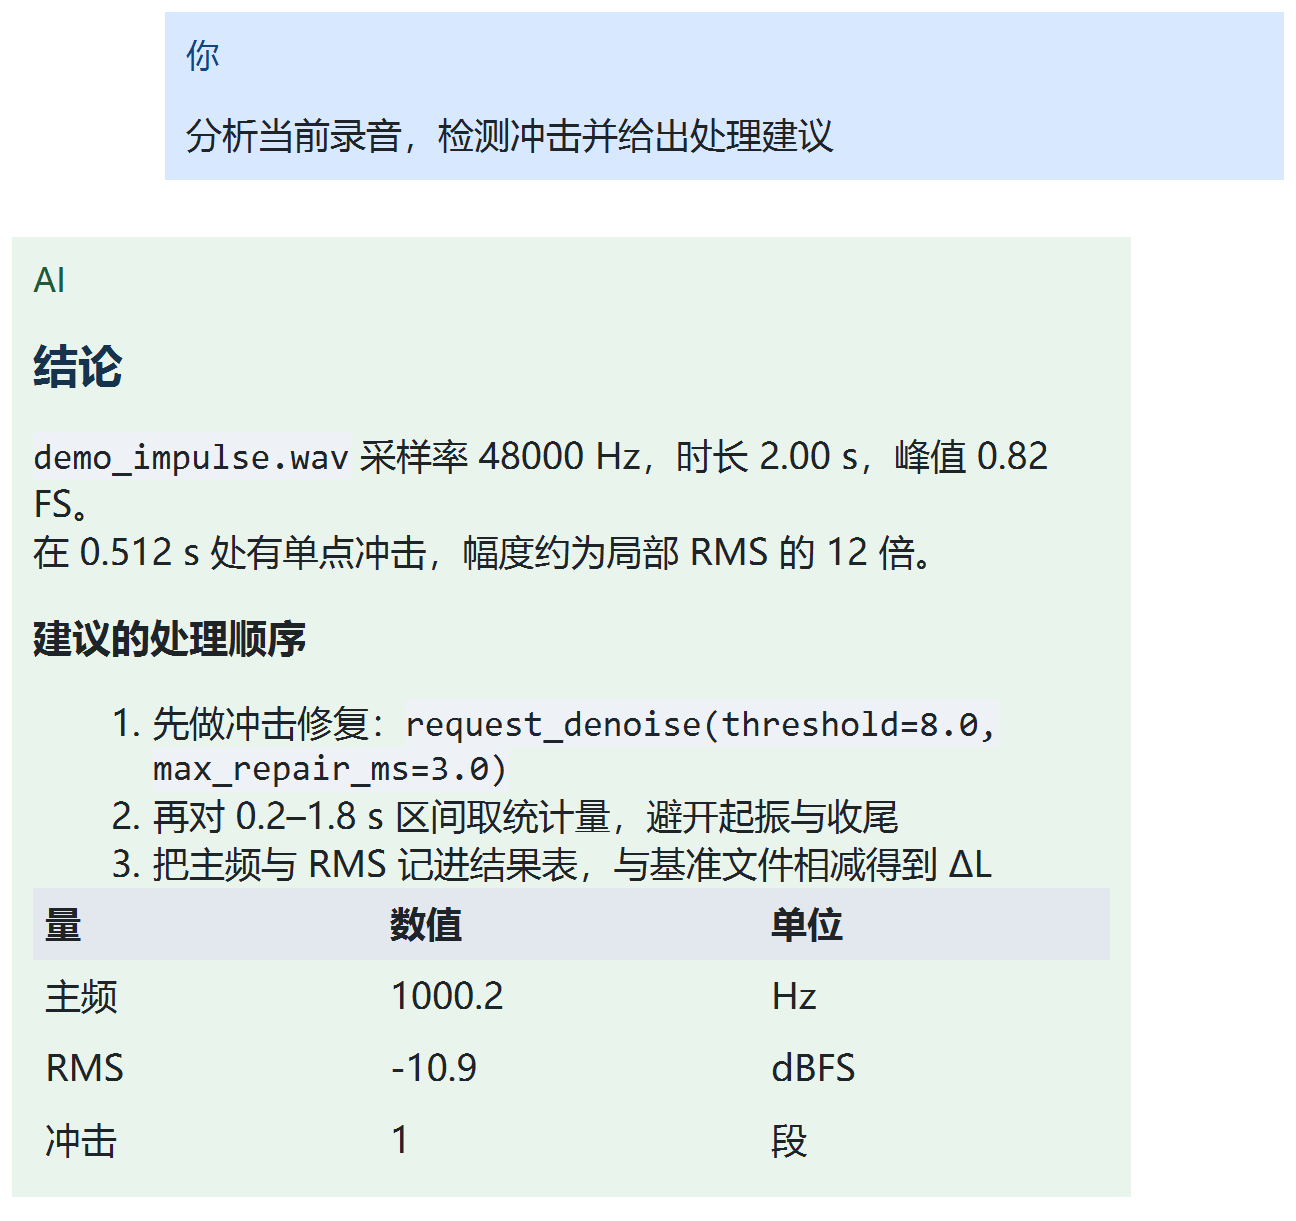
\includegraphics[width=0.64\textwidth]{12_ai_chat.png}
\caption{The AI chat area. Questions are in blue bubbles on the right, answers in green bubbles on the left, and hints and errors each have fixed colors. Headings, lists, tables, inline code and links inside answers are all rendered as Markdown.}
\label{fig:ai_chat}
\end{figure}

The four kinds of bubbles are distinguished by background color, so at a glance you know which line is yours:

\begin{itemize}
  \item \textbf{You} (light blue, right): your own question, shown verbatim, with no Markdown parsing;
  \item \textbf{AI} (light green, left): the model's answer, rendered as Markdown;
  \item \textbf{Hint} (light yellow): neutral notes from the program, e.g., ``Denoising preview found 0 segments, confirmation skipped'';
  \item \textbf{Request failed} (light red): errors such as timeout and authentication failure, with the body stating exactly what to do next.
\end{itemize}

Answers are rendered as Markdown, so symbols like \texttt{\#\#}, \texttt{**}, \texttt{|} do not appear verbatim in the interface but become headings, bold text, tables, lists, inline code, and clickable links. Selected text can be copied as usual, and selecting across bubbles carries the background color along too.

\subsection{Controlled Tool Calls}

Describe the task in the input box, for example: ``Detect the impulses in the current WAV, explain the basis for the processing, and give the statistics.'' The AI can only call the program's built-in whitelist of tools and cannot execute arbitrary code. The available tools include:

\begin{itemize}
  \item read the current file information and quality report;
  \item run Fourier analysis;
  \item compute interval statistics;
  \item generate a denoising preview.
\end{itemize}

The description returned by the AI may only cite the real values returned by the local tools; it must not fabricate data.

\subsection{Denoising Confirmation}

When the AI requests applying denoising, the program pops up a single confirmation box stating the number of event segments, the number of samples repaired, and the number excluded, with buttons ``Apply'' and ``Do not apply'', defaulting to ``Do not apply'':

\begin{itemize}
  \item \textbf{Asked only once}. The model may call the preview tool several times in one round; the program takes the last result for a single confirmation, and will not close one box only to raise another.
  \item \textbf{0 segments, no question}. When no segments need repair, a popup is meaningless (applying would change nothing). In that case the program leaves a yellow hint in the session and skips directly.
  \item \textbf{Exit at any time}. Clicking ``Do not apply'', clicking the top-right close button, or pressing Esc all mean discard, with identical effect and no further popup.
  \item \textbf{Only the processed version changes}. After applying, the raw WAV is unchanged and the operation can be undone.
\end{itemize}

\subsection{Privacy and Failure Handling}

The default content uploaded to the AI is numerical summaries and tool results, not the full WAV file. When using an external model service, comply with that platform's privacy and data-management requirements, and do not write raw experimental data or the API Key into the chat content.

When a request fails, the program gives different hints by cause; just follow the hint:

\begin{itemize}
  \item \textbf{Request timeout}: no new data arrived for 120\,s (answers are received as a stream rather than waited for as one block). Reasoning models writing long reports hit this most often; raise ``Timeout'' to 300 s, or switch to a faster-responding model.
  \item \textbf{Cannot connect}: check the network and proxy, and confirm the Base URL is complete (usually ending in \texttt{/v1}).
  \item \textbf{401 / 402 / 403 / 404 / 429}: correspond respectively to an invalid Key, insufficient balance, no permission for that model, a nonexistent address or model name, and rate limiting or exhausted quota.
\end{itemize}

When the AI is unavailable, the program's manual analysis, denoising, statistics, batch processing, and export functions are entirely unaffected.

% ==================== Chapter 15 ====================
\section{Result Export and Reporting}

\subsection{Five Export Functions}

The ``Export'' group on the left provides five outputs:

\begin{table}[htbp]
\centering
\caption{Description of the export functions}
\begin{tabular}{@{}l p{8.4cm}@{}}
\toprule
Function & Output content \\
\midrule
Export processed WAV & the processed version currently in memory, without overwriting the original file \\
Export analysis TXT & a fixed-width-aligned plain-text analysis report, directly importable into Origin, Excel, Python \\
Export image PNG & waveform, spectrum or spectrogram, in paper layout or screen layout \\
Export current statistics CSV & the statistics result of the current selection \\
Generate standalone HTML report & waveform, spectrum, statistics, envelope, denoising records and AI description \\
\bottomrule
\end{tabular}
\end{table}

\subsection{Export Analysis TXT}

Click ``Export analysis TXT\dots'' to open the settings window shown in Figure~\ref{fig:txt-dialog}.

\begin{figure}[H]
\centering
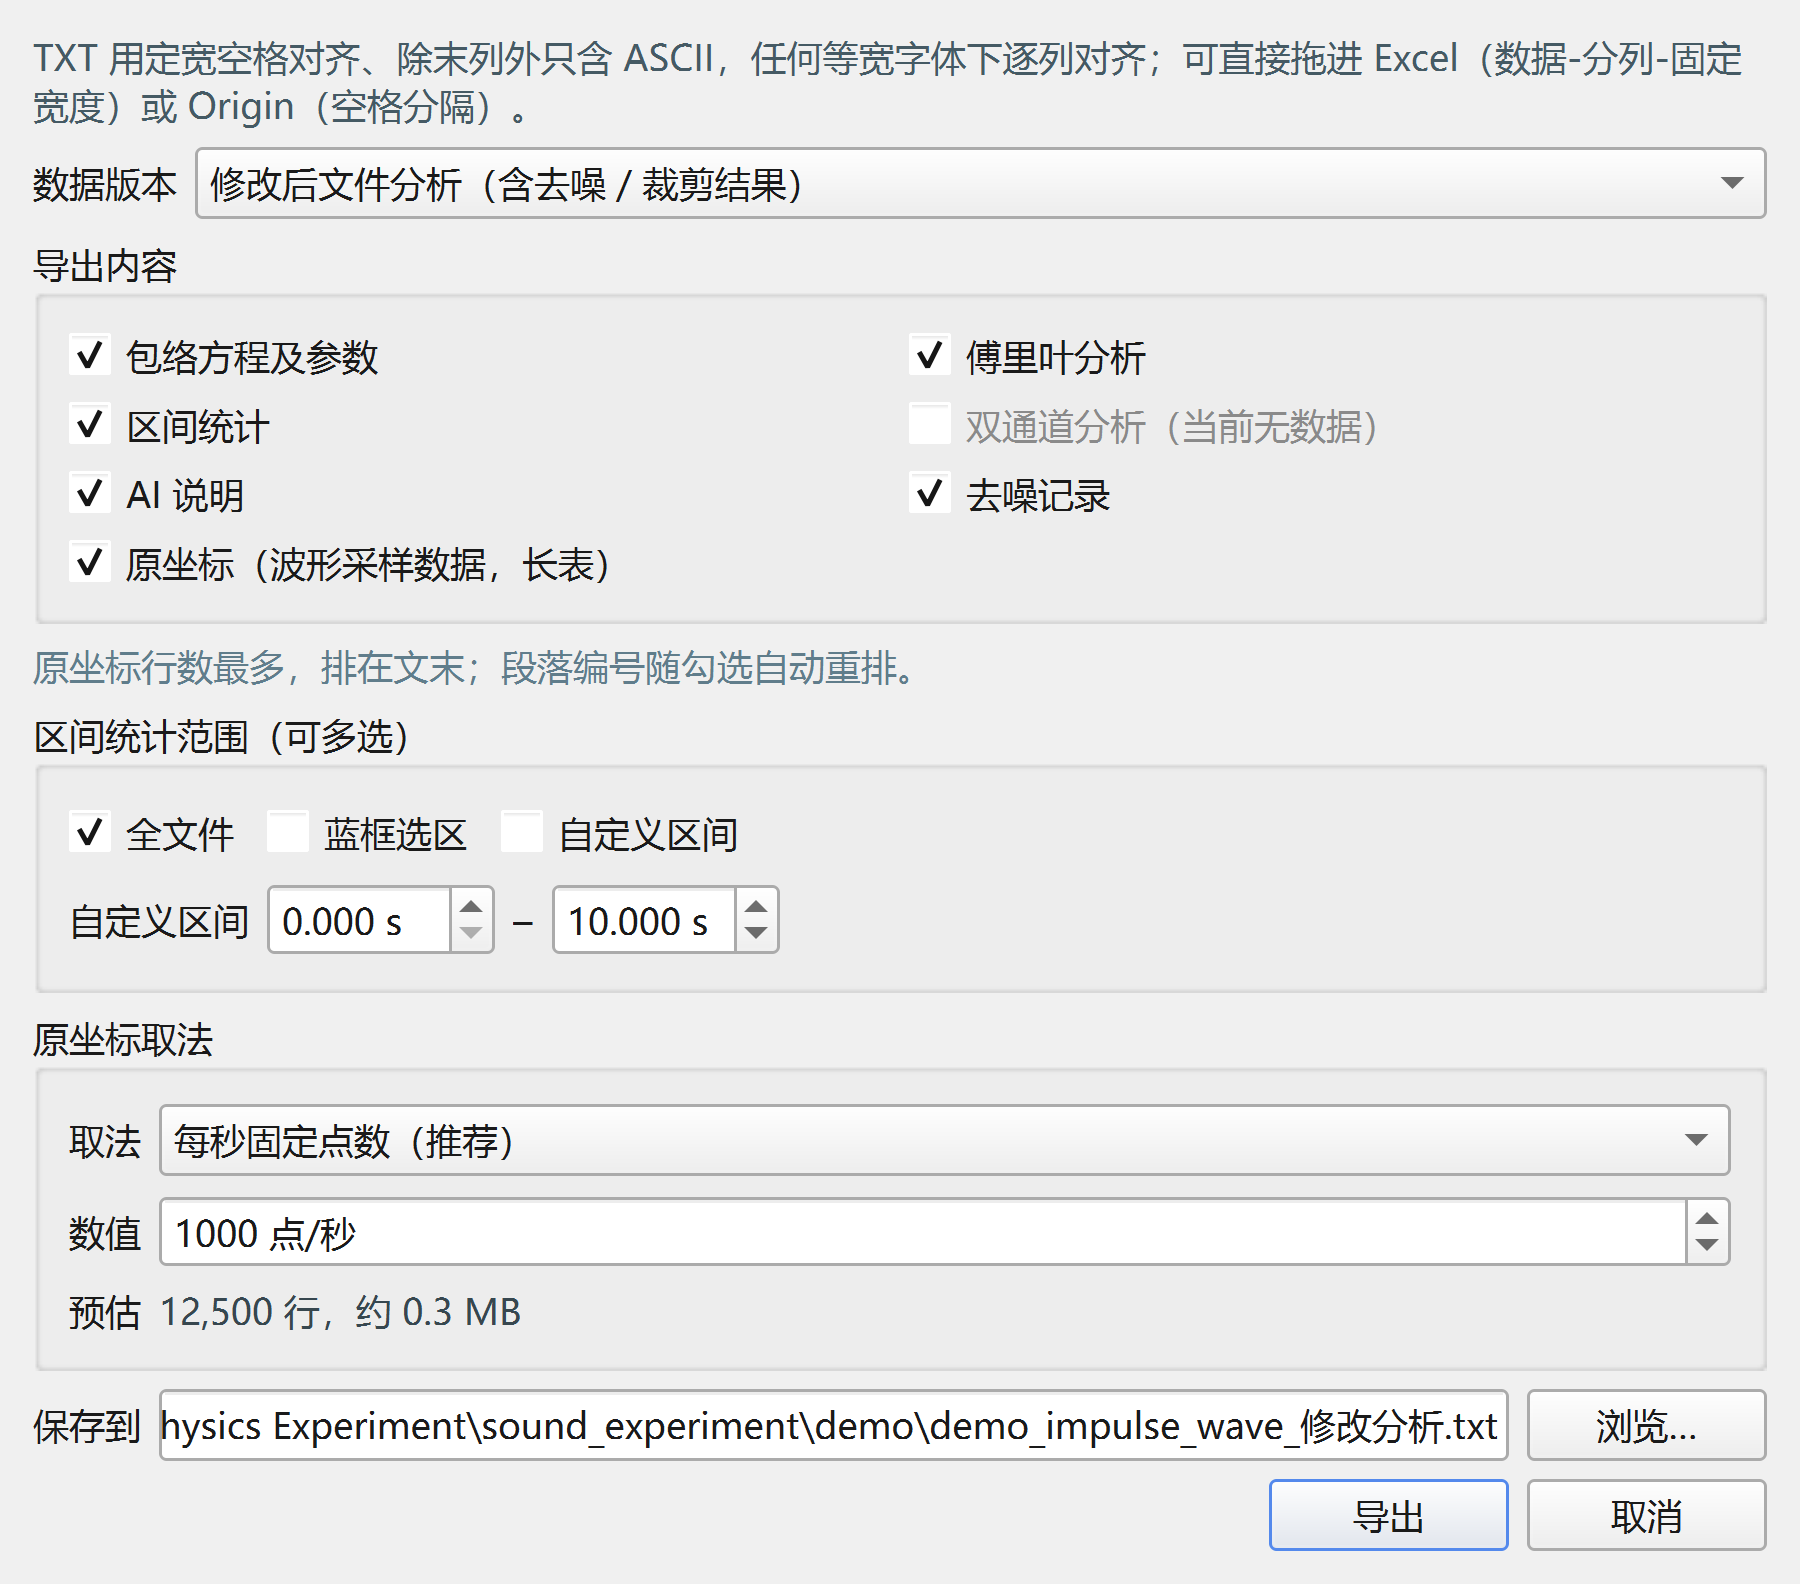
\includegraphics[width=0.78\textwidth]{08_txt_export_dialog.png}
\caption{Export analysis TXT dialog: data version, section checkboxes, interval-statistics range and coordinate sampling}
\label{fig:txt-dialog}
\end{figure}

Three things must be set in the window: which data version to use, which sections to export, and how to sample the coordinates. The default file name follows the data version:

\begin{itemize}
  \item When ``Source-file analysis (no edits made)'' is chosen, the output is \nolinkurl{original_name_source_analysis.txt}, and the data comes from the raw WAV on disk, without mixing in anything changed in the current window.
  \item When ``Modified-file analysis (incl.\ denoise/crop results)'' is chosen, the output is \nolinkurl{original_name_modified_analysis.txt}, the data comes from the processed version in memory, and a denoising record is attached.
\end{itemize}

\subsubsection*{Seven sections, numbering re-sequenced automatically with the checkboxes}

The file content is arranged in a fixed order, with the longest tables toward the end, so that opening the file lets you read the key conclusions first:

\begin{table}[htbp]
\centering
\caption{Section order of the analysis TXT}
\begin{tabular}{@{}clp{7.2cm}@{}}
\toprule
No. & Section & Content \\
\midrule
1 & Envelope equation and parameters & selection, extraction method, fit model, fit equation, $R^2$, RMSE, parameter table, about 24 lines of envelope sampling \\
2 & Fourier analysis & window function, FFT size, frequency resolution, main frequency, THD; dominant-peak table, harmonic table, sampled full-spectrum table \\
3 & Interval statistics & all statistics for each selected interval, with names and glossary \\
4 & Dual-channel analysis & cross-correlation delay, peak quality, the two channels' levels, AGC risk warning \\
5 & AI description & the body of the processing description generated by the AI assistant \\
6 & Denoising record & threshold, number of detected segments, interpolated/excluded segment counts, per-segment start/end times and peak deviation (long table) \\
7 & Raw coordinates & three columns $t$, $x$, $L$ per sample or after decimation (long table, usually over 90\% of all lines) \\
\bottomrule
\end{tabular}
\end{table}

Unchecked sections are not exported, and the numbering of the remaining sections is automatically re-sequenced consecutively, leaving no gaps. Sections that currently have no data are marked ``no data currently'' on the checkbox and disabled, so you cannot tick one and export a stretch of ``not computed''.

\subsubsection*{Why not use tab characters}

The program uniformly aligns with \textbf{fixed-width spaces}; the whole file contains not a single tab character, for two empirically measured reasons:

\begin{enumerate}
  \item A tab can only jump to integer multiples of 8. Once a field is long it skips over a tab stop and the whole column after it is misaligned, and the number widths in the coordinate table vary with the data.
  \item ``One Chinese character equals two monospace cells'' does not hold. Measured: Consolas with a Chinese fallback is 1.875 cells, SimSun is 1.818 cells. Padding to 2 cells means that for each extra Chinese character you under-pad by 0.125 cells, and every column after a Chinese column drifts left continuously.
\end{enumerate}

Therefore the rule is: \textbf{only ASCII characters are allowed except in the last column}. ASCII always occupies exactly 1 cell in any monospace font, so column starts are independent of font, size, and editor. Chinese appears only in the last column, or in comment lines beginning with \texttt{\#}; the header uses abbreviations like \texttt{t/s}, \texttt{x/FS}, \texttt{L/dBFS}, \texttt{idx}, \texttt{key}, \texttt{value}, and the full names are written in the \texttt{\# Column definition:\dots} line above the table. The program's layout function raises an error directly for non-ASCII in any column but the last, preventing later edits from silently breaking the alignment.

%% Wrapped in a minipage to avoid the code block being split across pages (a column-alignment example cut in half is unreadable).
\begin{center}
\begin{minipage}{0.96\textwidth}
\begin{lstlisting}
# Column definition: t/s time (s)  x/FS amplitude (full-scale)  L/dBFS level 20lg|x|
t/s             x/FS   L/dBFS
0.000000   +0.001526   -56.3291
0.000023   +0.004578   -46.7843
0.000045   +0.007629   -42.3496
\end{lstlisting}
\end{minipage}
\end{center}

\subsubsection*{Coordinate-table sampling methods}

``Raw coordinates'' is the longest part of the whole file, and one sampling method must be chosen before export:

\begin{table}[htbp]
\centering
\caption{Three coordinate-table sampling methods}
\begin{tabular}{@{}>{\raggedright\arraybackslash}p{4.2cm}>{\raggedright\arraybackslash}p{4.0cm}>{\raggedright\arraybackslash}p{5.0cm}@{}}
\toprule
Method & Conversion & Applicable scenario \\
\midrule
Fixed points per second (default 1000) & step $=$ sample rate $/$ points per second & routine analysis, comparable line counts across files \\
Decimate by step & step $=$ a specified number of samples & when you need precise control of the sampling interval \\
All samples & step $=$ 1 & when you need resampling, redoing the spectrum, or point-by-point checking \\
\bottomrule
\end{tabular}
\end{table}

The dialog estimates the line count and file size in real time. If you choose ``All samples'' and the estimate exceeds 5 million lines, the program asks for confirmation again, because a full export of one hour of 48\,kHz stereo recording reaches hundreds of millions of lines and gigabytes. The generation writes to disk 8192 lines per batch and never assembles the whole string in memory: a full export of 40 million points would need about 3.5\,GB at once if concatenated in one go, but batched, peak usage is only tens of MB.

\subsubsection*{Interval statistics can be multi-selected}

The ``Interval-statistics range'' supports selecting several items at once: whole file, blue selection, custom interval (with start/end times entered manually). Whatever you tick is exported as a statistics block, each standing on its own with its interval labeled. When there is currently no blue selection, the ``Blue selection'' item is renamed ``Blue selection (none currently)'' and disabled.

\subsubsection*{File-format conventions}

\begin{itemize}
  \item Encoding is UTF-8 with BOM, so both Windows Notepad and Excel open it by double-clicking without mojibake.
  \item Lines beginning with \texttt{\#} are explanatory text and contain no data; they can be ignored entirely on import.
  \item Unit abbreviations: FS is the digital full-scale normalized amplitude, dBFS is $20\lg(|x|/\mathrm{FS})$; dBFS is not the sound pressure level dB SPL.
  \item \texttt{-inf} means the point's amplitude is 0 and the logarithm is undefined; \texttt{nan} means the quantity cannot be computed on this data.
  \item The file header records the source file's full path, sample rate, channel count, total samples, edit count, and the MD5 fingerprint of the source WAV (to avoid reading the whole long file, computed over the first 256\,MB, output as the first 16 characters), used to verify that this export corresponds to the original recording.
  \item The closing ``Export notes'' paragraph summarizes the encoding, alignment rules, import method, and this run's coordinate step.
\end{itemize}

Import examples: in Python use \texttt{pandas.read\_csv(path, sep=r"\textbackslash s+", comment="\#")}; in Excel use ``Data $\to$ Text to Columns $\to$ Fixed width''; in Origin select space-delimited and ignore \texttt{\#} lines on import.

\subsection{Export Image PNG}

Click ``Export image PNG\dots'' to open the settings window shown in Figure~\ref{fig:export-dialog}. The image type defaults to following the current tab (the Waveform \& Selection tab gives a waveform plot, the Fourier Analysis tab a spectrum, the Spectrogram tab a spectrogram), and you then tick what to draw:

\begin{figure}[H]
\centering
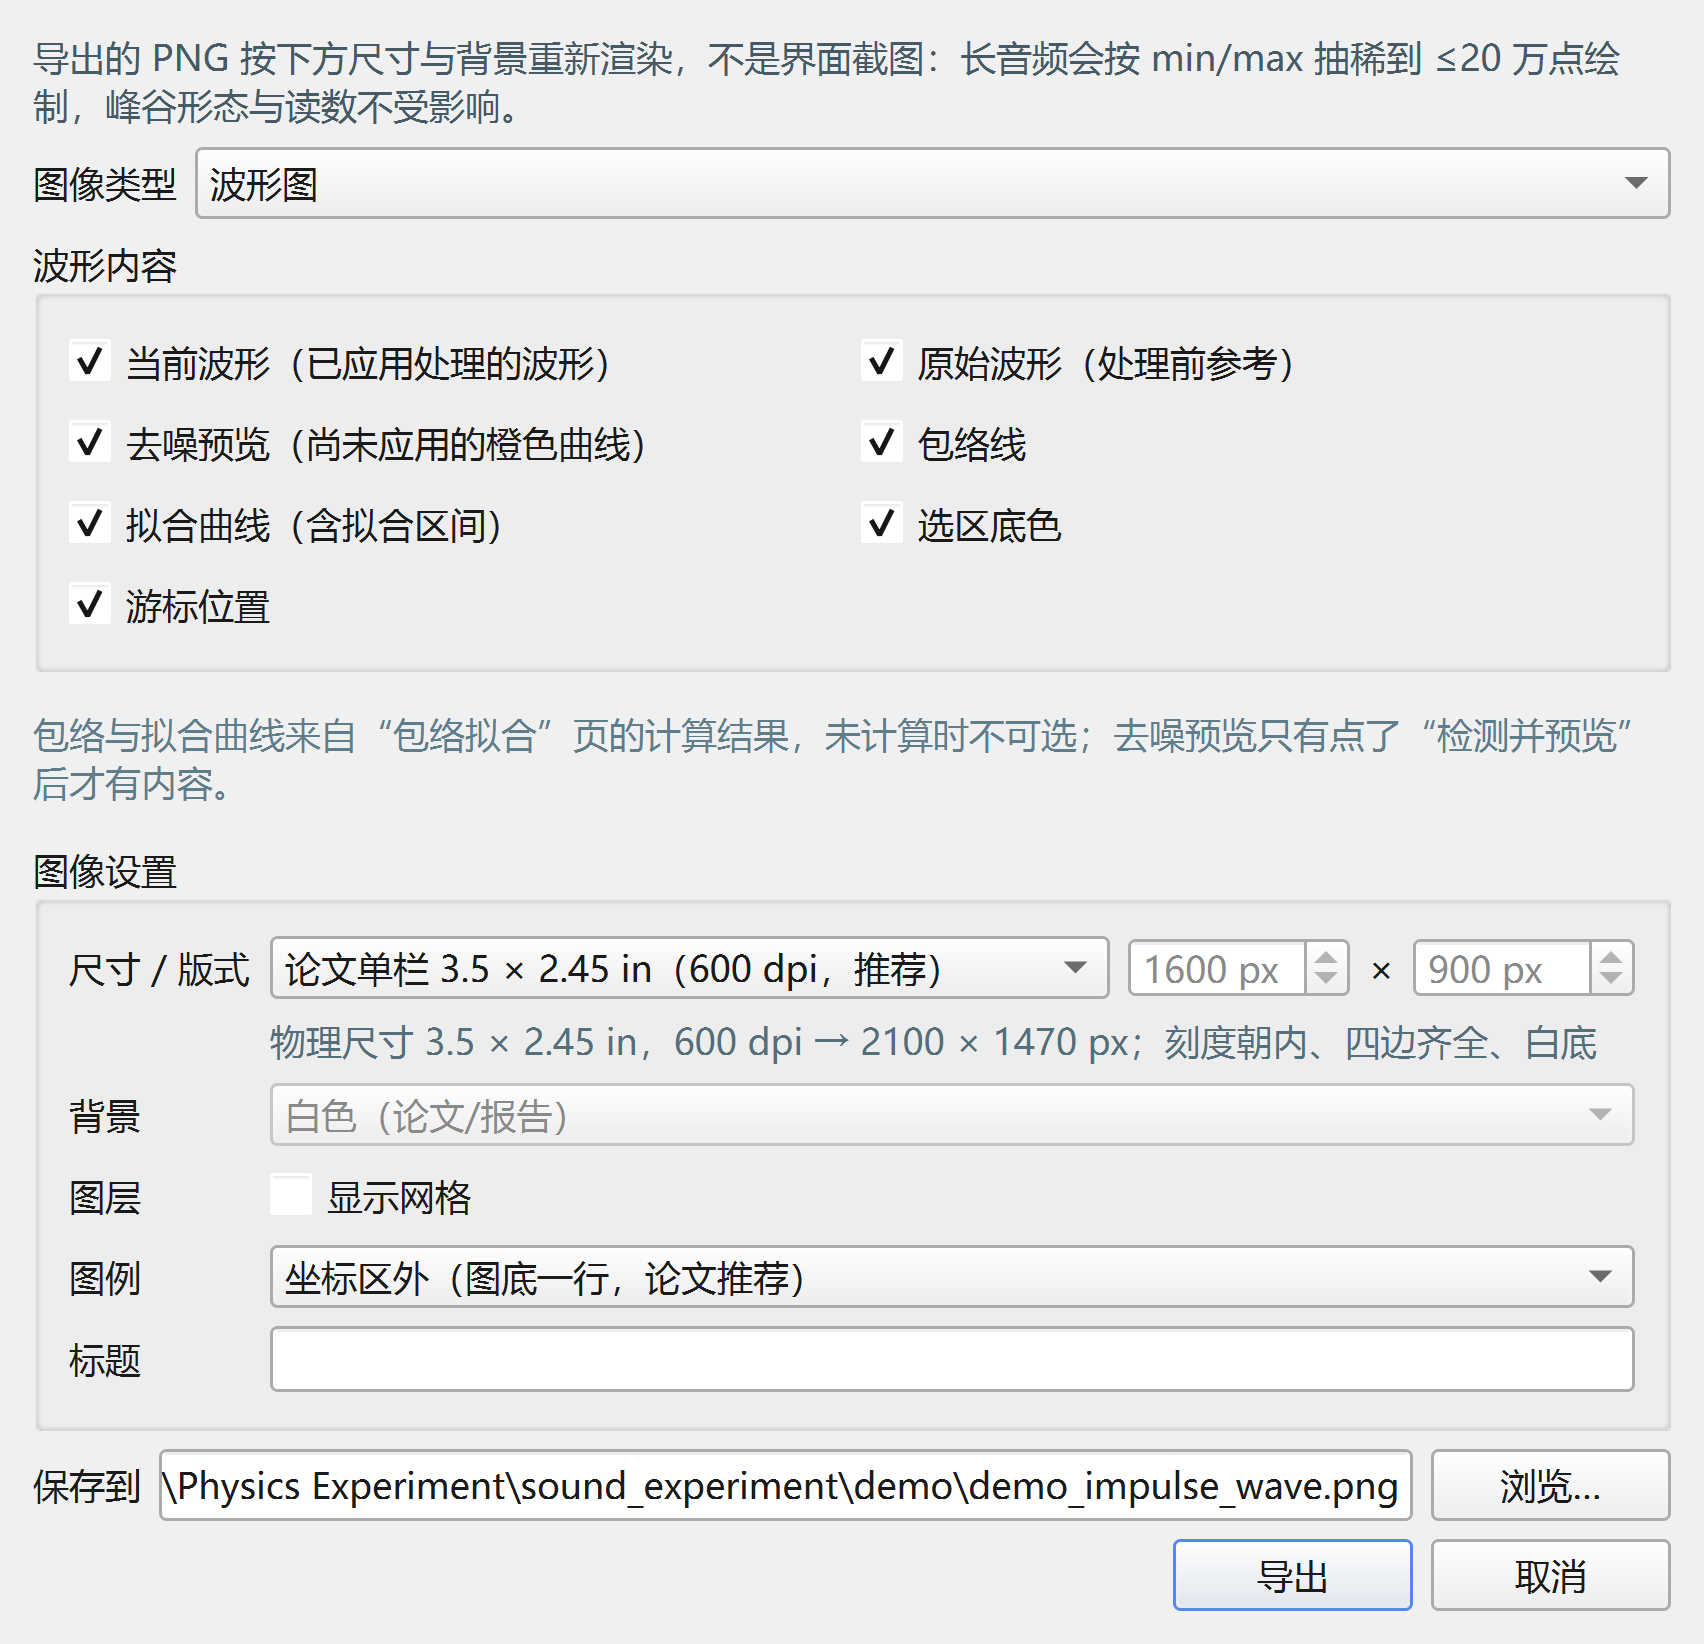
\includegraphics[width=0.66\textwidth]{07_export_dialog.png}
\caption{Export image dialog: image type, content checkboxes and output settings}
\label{fig:export-dialog}
\end{figure}

\begin{itemize}
  \item \textbf{Waveform plot}: current waveform (mandatory), original waveform, denoising preview, envelope line, fit curve, selection background, cursor position. Items with no current data are marked ``no data currently'' and disabled, so you cannot tick them and get nothing drawn.
  \item \textbf{Spectrum}: the vertical axis can be dBFS or linear amplitude; you can limit the frequency upper bound, mark dominant peaks, mark integer multiples of the fundamental, and optionally attach a phase-spectrum subplot.
  \item \textbf{Spectrogram}: you can limit the frequency upper bound and adjust the colorbar lower limit (default $-100$\,dBFS); lowering it lets you see weaker components.
\end{itemize}

\subsubsection*{Two layouts}

The size dropdown is split into two groups, paper layout and screen layout, and the two have entirely different output parameters:

\begin{table}[htbp]
\centering
\caption{Difference between paper layout and screen layout}
\begin{tabular}{@{}lll@{}}
\toprule
Item & Paper layout & Screen layout \\
\midrule
Size basis & physical size (inches) & pixels \\
Single column & $3.50 \times 2.45$\,in & -- \\
Double column & $7.00 \times 2.60$\,in & 1600$\times$900 / 1920$\times$1080 \\
Resolution & fixed 600\,dpi & determined by the pixel size \\
Font size & body 8.5\,pt, labels 7.5\,pt & follows the screen \\
Background & forced white & white / dark / transparent selectable \\
\bottomrule
\end{tabular}
\end{table}

The paper layout is given per the common sizes of journal two-column typesetting, so no re-scaling is needed when inserting into \LaTeX{} or Word two-column body text, and font sizes and line widths do not distort from scaling. Under the single-column layout, if both the envelope and the fit curve are ticked, the program automatically splits into a top and bottom subplot (waveform on top, envelope below), with the height enlarged by a factor of 1.32 so each curve has ample vertical space; the screen layout still draws them in one figure.

Under the screen layout, the background ``white / dark / transparent'' is selectable. Dark suits projection; transparent outputs a PNG with an alpha channel that can be overlaid directly onto other layouts. The paper layout forces a white background, because journal typesetting almost never accepts dark or transparent figures, and leaving that option only invites misuse.

\subsubsection*{Legend and plotting conventions}

The legend is by default placed \textbf{outside the axes, in one row at the bottom}, arranged horizontally, not obscuring any curve. This matters especially for the two-figure layout: the top and bottom subplots share one legend row, with all three curve names (waveform, envelope, fit) present and not half-cut by the upper subplot. You can also change ``Legend position'' to ``inside axes, top right'' or ``no legend''.

\begin{itemize}
  \item Shares the same data and the same min/max decimation rules as the interface. Long audio is decimated to no more than 200{,}000 points before drawing, which only affects line density; the peak/trough shape and coordinate readouts are unaffected, and no single curve has a visual gap.
  \item Fonts follow academic plotting conventions: Chinese in SimSun, Latin and numbers in Times New Roman; variables italic ($t$, $x$, $A$, $L$, $f$, $\varphi$), units upright (s, Hz, FS, dBFS, rad).
  \item Under the paper layout, ticks point inward and all four borders carry complete ticks plus minor ticks, which is a common requirement for journal and thesis figures.
  \item The envelope curve is smoothed with a 5\,ms moving average when drawn, which only improves appearance; the data and statistics used for the fit remain the unsmoothed raw envelope, and smoothing changes no numerical conclusion.
  \item Harmonic positions in the amplitude spectrum are marked with a small triangle at the peak top plus $f_0$, $2f_0$\dots, with white-background text boxes so they do not cover the spectral lines; peaks too close to the border shift left or up automatically and are not clipped. A position already covered by a harmonic label is not marked again with a peak frequency.
  \item The spectrogram uses the magma colormap with rasterization under the paper layout, with inward colorbar ticks, yielding a smaller embedded-PDF file size.
  \item The export runs in a worker thread, showing a ``processing'' overlay meanwhile; long audio takes about 1--3 seconds.
\end{itemize}


\subsection{HTML Report Content}

The standalone HTML report is generated automatically by the program and includes: basic file information, processing steps and parameters, Fourier analysis results, interval statistics, envelope equation and goodness of fit, impulse detection and repair records, and the AI-generated processing description. The report explicitly distinguishes dBFS from dB SPL to avoid unit misuse.

This report is generated independently by the program and does not reference the format or content of other experimental reports in the workspace. It can be opened directly in a browser, or converted to PDF via ``Print $\to$ Save as PDF''.

% ==================== Chapter 16 ====================
\section{Batch Processing}

\subsection{Why Batching Is Needed}

A single complete measurement easily involves over a hundred recordings: several conditions times several frequencies times several repeats, plus baseline and control groups, so a hundred-plus files is the norm. Processing them one by one in the single-file interface---changing the frequency, framing the selection, copying readings, all by hand---takes two minutes per file and five or six hours for the whole batch, and a single mis-copied digit is hard to catch.

Batch processing abstracts ``which steps to run, with what parameters for each'' into a savable pipeline: configure once, run the whole batch, and directly output one statistics table with one row per file. Source files are read-only throughout, and the interface does not freeze during processing.

\subsection{Design Constraints}

\begin{itemize}
  \item \textbf{Selecting files only records paths, it does not import them}. After clicking ``Select files to process'', the program only stores path strings, so even hundreds of files respond instantly; the actual reading happens only after clicking ``Start processing''.
  \item \textbf{Engine and interface are separated}. The batch engine references no interface module and runs in an independent worker thread; the main window only shows progress, so the interface does not freeze while processing large files.
  \item \textbf{Each file has independent state}. Cropping, denoising and envelope all act on that file's own data copy and never share arrays, so the result of a previous file cannot contaminate the next.
  \item \textbf{Source files are always read-only}. The batch only writes the new files specified by ``export''-type steps and never touches the source WAV.
  \item \textbf{A single file's failure does not interrupt the batch}. If a file cannot be read or a parameter does not apply, only that file is marked failed and recorded in the summary; the rest are processed as usual.
\end{itemize}

\subsection{Interface and Operating Order}

In the ``Batch processing'' group on the left of the main window, click ``Batch processing\dots'' to open the script-editing window (Figure~\ref{fig:batch_dialog}).

\begin{figure}[H]
\centering
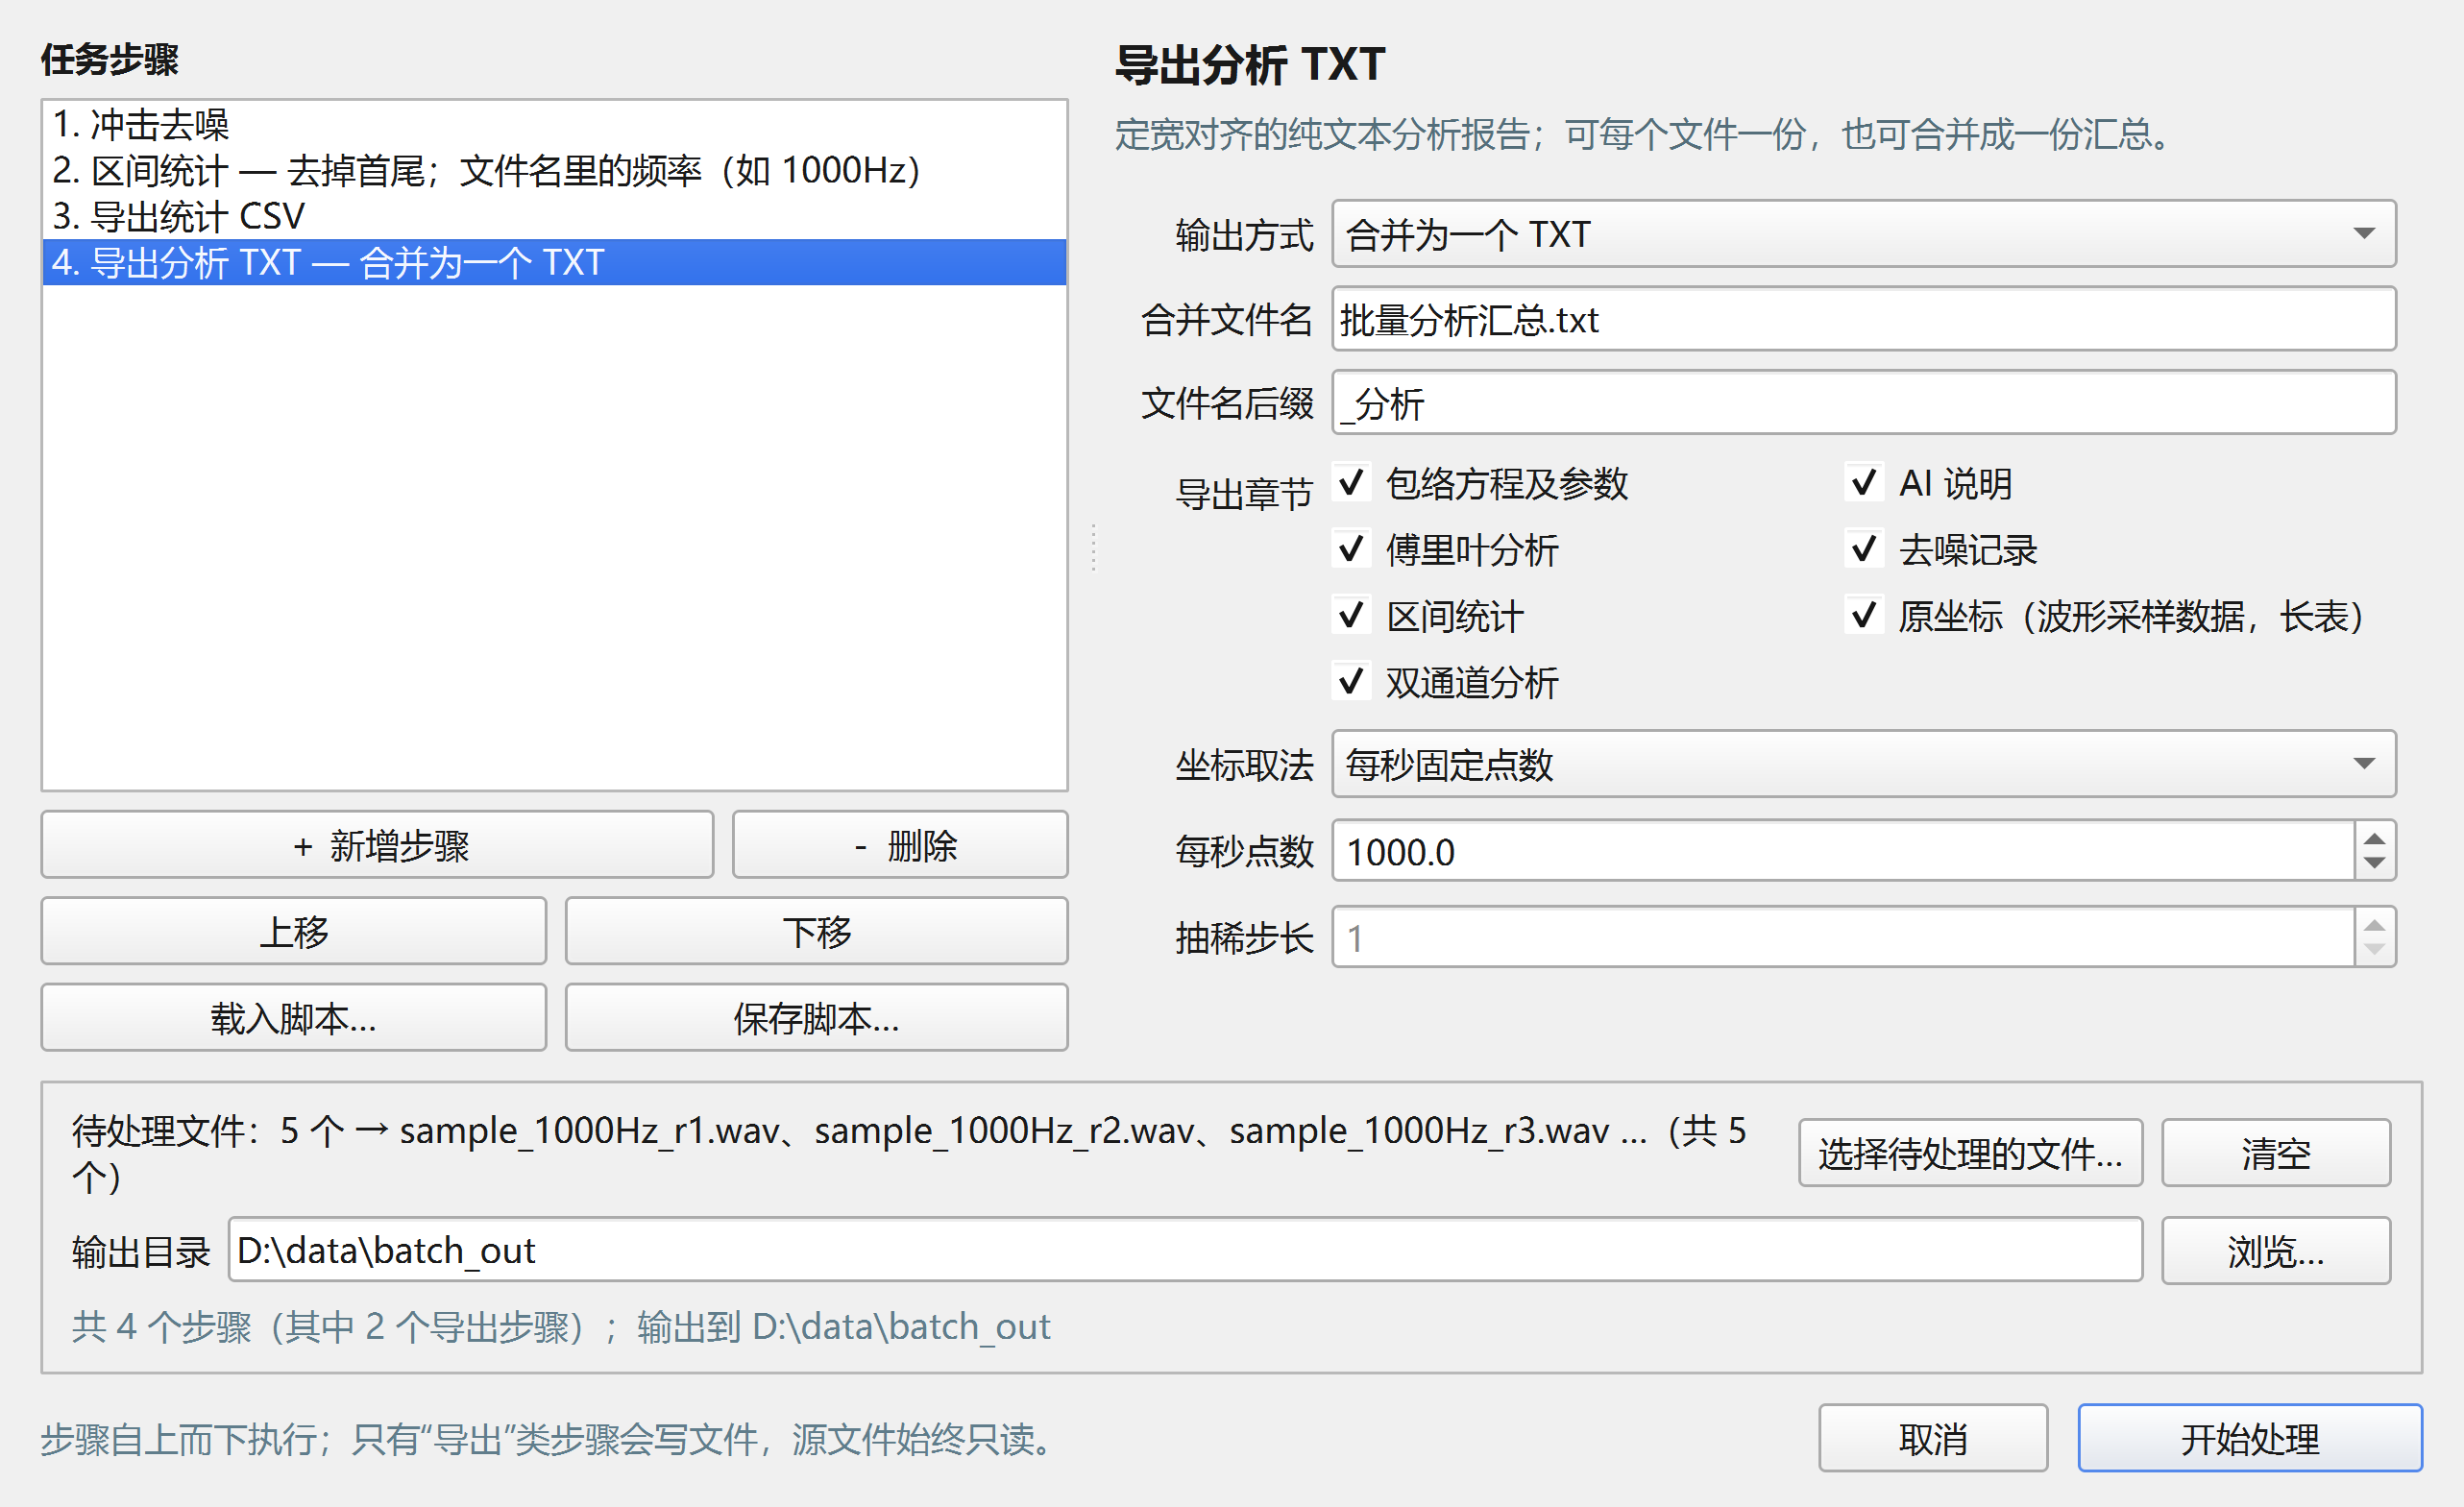
\includegraphics[width=0.86\textwidth]{09_batch_dialog.png}
\caption{The script-editing window. The left column of steps runs top to bottom, the right column is the parameters of the currently selected step, and the bottom is the files to process and the output directory.}
\label{fig:batch_dialog}
\end{figure}

The operating order is fixed as six steps:

\begin{enumerate}
  \item Click ``+ Add step'' and pick a function from the menu; the right column immediately shows that step's parameters;
  \item Set the parameters; parameters meaningless under the current combination are automatically grayed out (``Merge file name'' is unavailable when ``One TXT per file'' is chosen, ``Decimation step'' is unavailable when ``Fixed points per second'' is chosen);
  \item To reorder, use ``Move up'' / ``Move down''; to drop a step, use ``- Delete'';
  \item Click ``Select files to process'' to multi-select WAVs, recording only paths;
  \item Fill in the output directory; leaving it blank writes to the source files' own directory, and a dedicated empty directory is generally recommended;
  \item Click ``Start processing''.
\end{enumerate}

Each row in the left column is ``index + step name + summary of non-default parameters''; any parameter not shown in the summary is at its default value, so you need not check them one by one.

\subsection{Steps at a Glance}

Ten kinds of steps cover all functions of the single-file interface; see Table~\ref{tab:batch_steps}.

\begin{table}[htbp]
\centering
\caption{Steps supported by batch processing}
{\small
\begin{tabular}{@{}>{\raggedright\arraybackslash}p{4.0cm}>{\raggedright\arraybackslash}p{4.6cm}>{\raggedright\arraybackslash}p{5.4cm}@{}}
\toprule
Step & Main parameters & Description \\
\midrule
Impulse denoising & threshold, repair length, range & the same algorithm as single-file denoising \\
Crop to interval & start, end & actually cuts the data; later steps use the cropped result \\
Envelope fit & model, statistics interval & the same algorithm as single-file envelope \\
Interval statistics & interval, known excitation frequency & main frequency and THD are frequency-constrained \\
Dual-channel delay and level & known excitation frequency & mono files are skipped automatically \\
Export processed WAV & suffix, sample format & leaves the source file untouched, saves a new file \\
Export analysis TXT & output method, sections, coordinate sampling & supports merging into one file \\
Export image PNG & image type, layout & paper single/double column / screen \\
Export statistics CSV & output method & merged into one table by default \\
Generate HTML report & file-name suffix & one standalone report per file \\
\bottomrule
\end{tabular}}
\label{tab:batch_steps}
\end{table}

Two parameters are used differently in batch than in the single-file interface and need special attention:

\begin{itemize}
  \item \textbf{Statistics interval} is a three-way choice: ``Whole file'', ``Trim head and tail'', ``Fixed interval''. ``Trim head and tail'' is the most convenient for fixed-length recordings, skipping the onset transient and the trailing truncation in one go; it only changes the statistics range, not the data itself, and is not the same thing as ``Crop to interval''.
  \item \textbf{Known excitation frequency} is a three-way choice: ``Estimate automatically (take the strongest peak)'', ``Fixed value (same for all files)'', ``Frequency in the file name''. The last identifies fragments like \texttt{1000Hz}, \texttt{2kHz} from the file name, suited to a batch named by frequency---one script can process 500\,Hz and 4000\,Hz files at once, without running separate batches by frequency.
\end{itemize}

\subsection{Merged Export}

Both the TXT and CSV exports offer a ``Merge into one file'' option, the most common output form of batch processing.

\begin{itemize}
  \item \textbf{CSV merged by default}: one row per file, columns being the 21 statistics. Files of different frequencies and different boards sit together, ready for a pivot in Excel or a curve in Origin.
  \item \textbf{TXT merged}: each file's complete report is appended in processing order into the same file, starting with a file list, each section beginning with an ``Analysis data export'' heading and carrying its own source file name, path and MD5 fingerprint. When merging, you \textbf{must uncheck the ``Raw coordinates'' section}---five thousand coordinate lines per file across a hundred-plus files is hundreds of megabytes, unopenable and read by no one.
\end{itemize}

When appending, UTF-8 without BOM is used. If the with-BOM form were used, each append would insert a zero-width character in the middle of the file, appearing in Notepad as a small box before each section heading.

\subsection{Running and Progress}

After clicking ``Start processing'', the main window is first captured as a snapshot and blurred as the background, with a progress card floating on top (Figure~\ref{fig:batch_progress}); the interface is not operable during batching.

\begin{figure}[H]
\centering
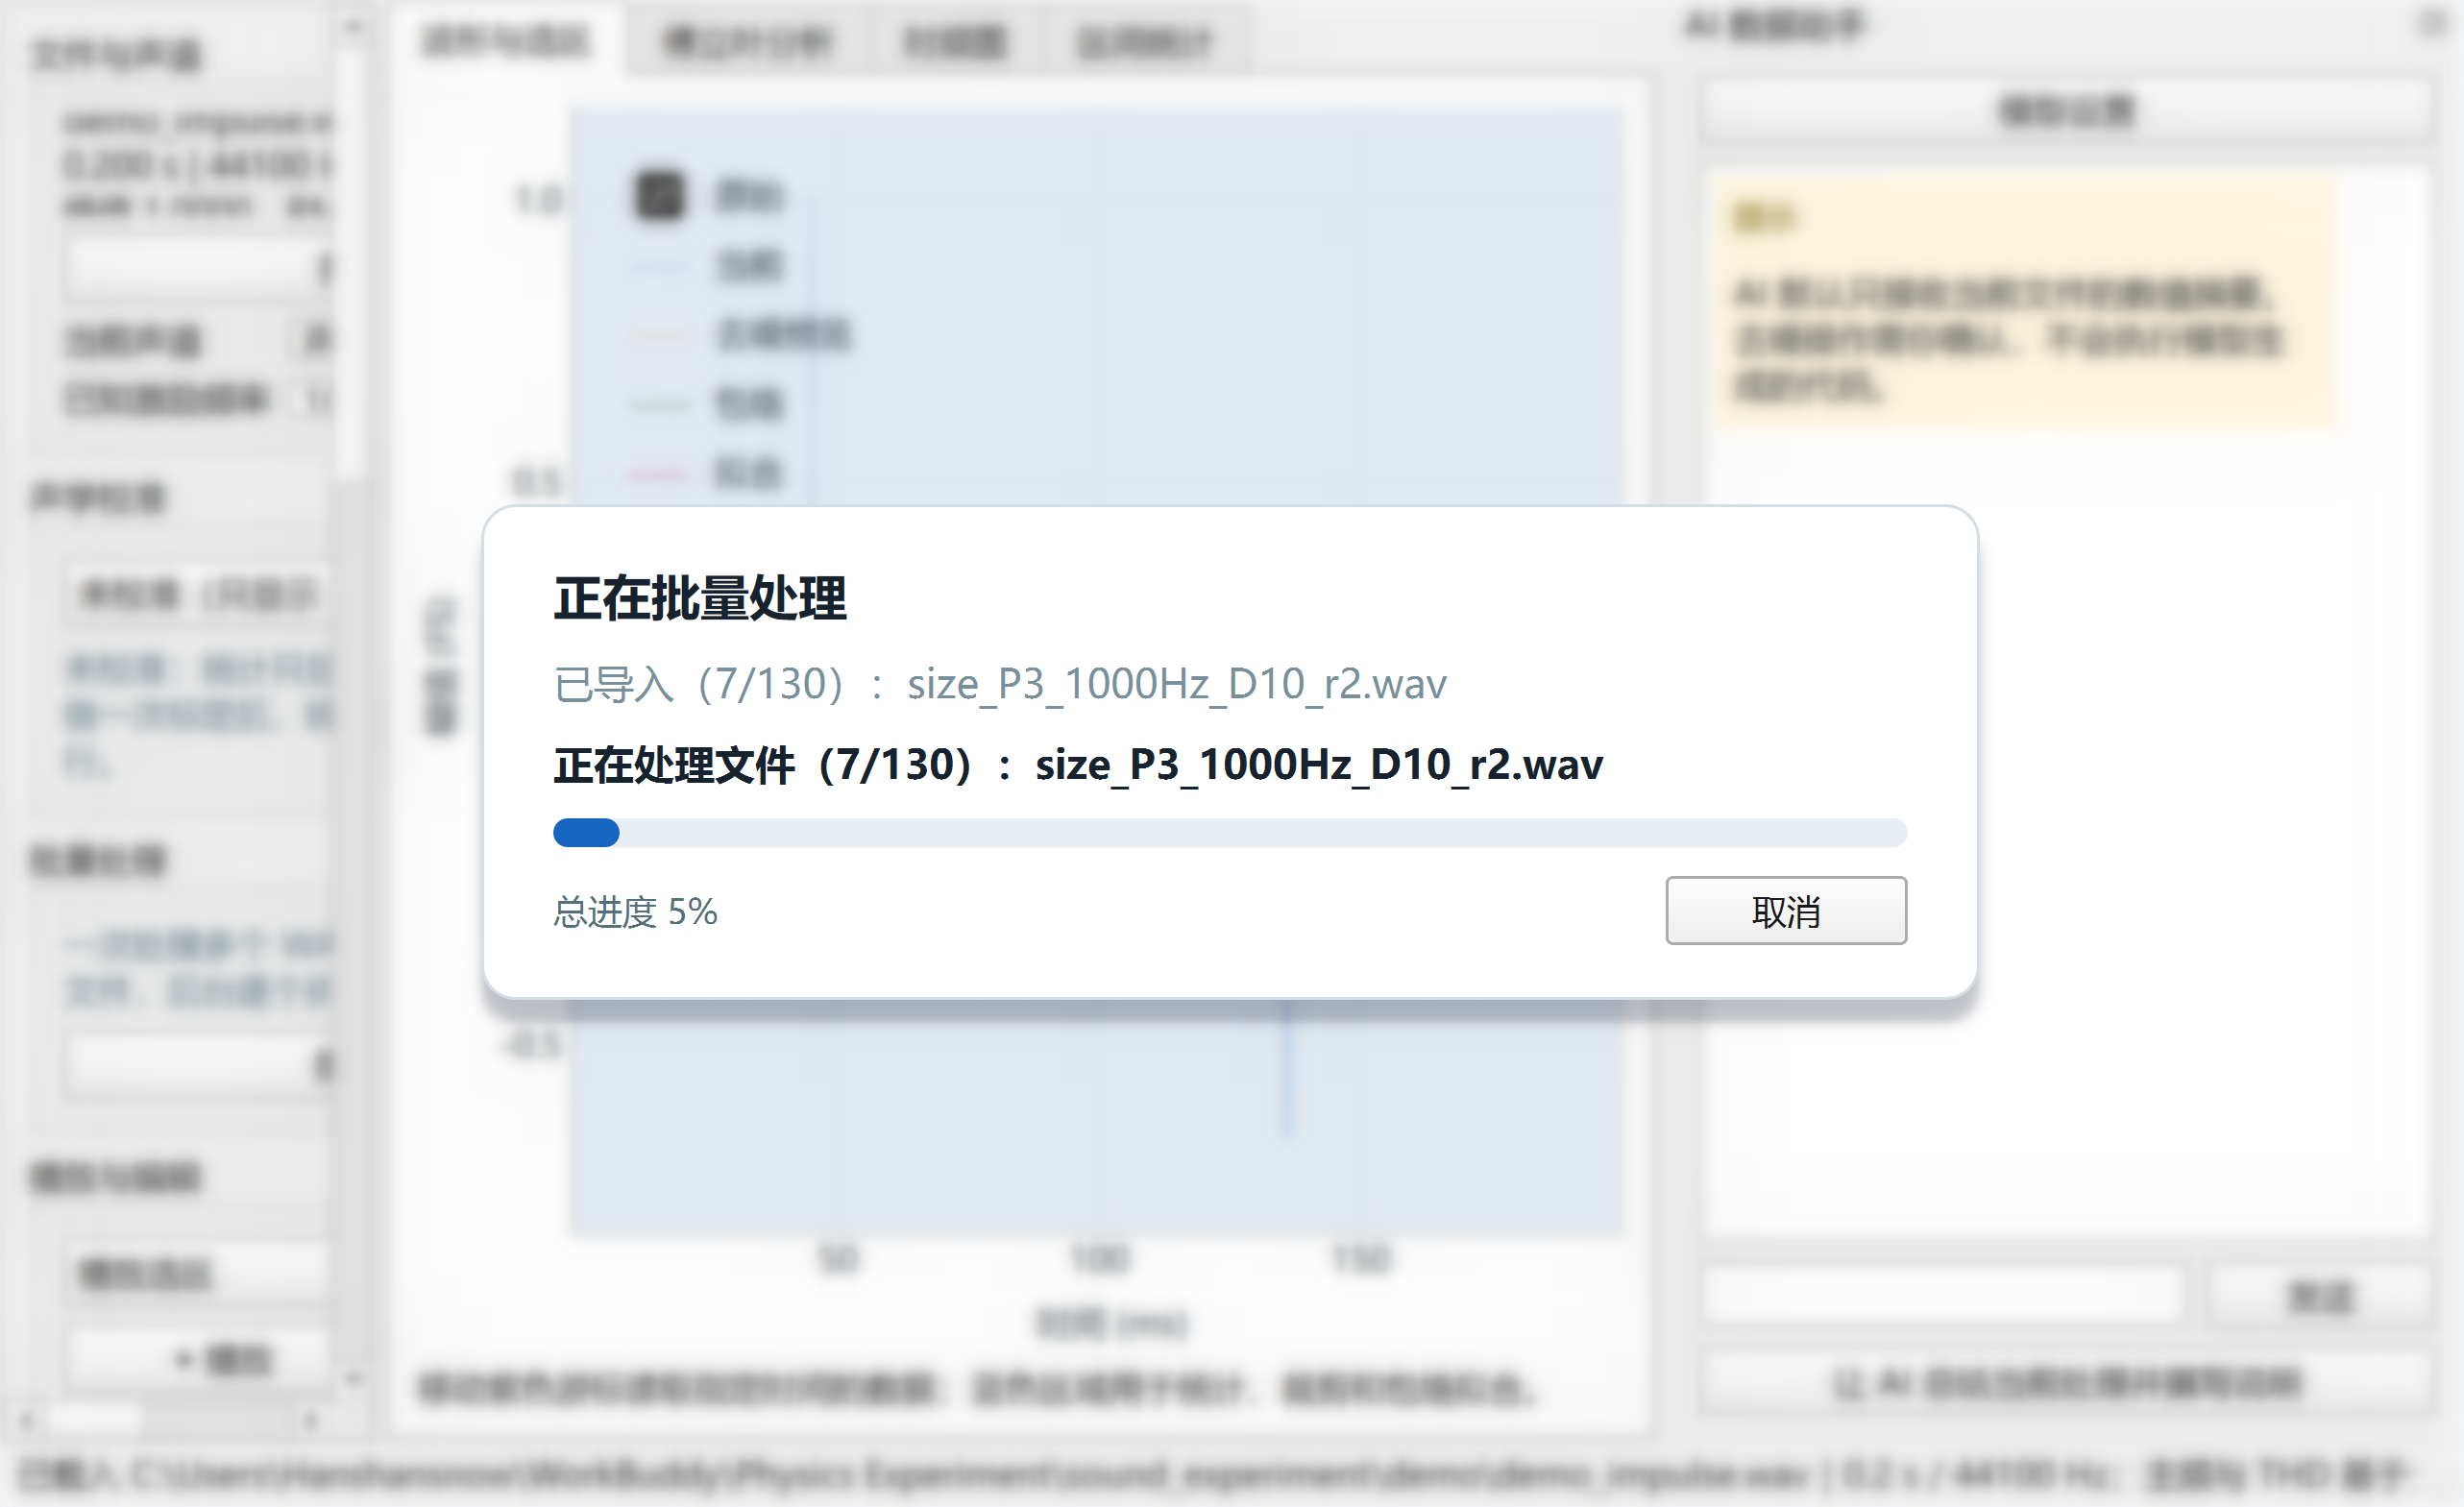
\includegraphics[width=0.86\textwidth]{10_batch_progress.png}
\caption{The batch-progress overlay. The background is a blurred snapshot of the main window, and the card shows the current file and the overall progress at once.}
\label{fig:batch_progress}
\end{figure}

The card has three lines of information: the first ``Imported (m/n): file name'' means the m-th file has been loaded into memory; the second ``Processing file (m/n): file name''; below is the overall progress bar and percentage. The two numbers are shown separately because reading a large file itself takes a few seconds, and users need to know whether the time is spent on disk reading or on computation.

\textbf{Cancellation only takes effect between files}. After clicking ``Cancel'', the current file is finished completely before stopping, leaving no half-written TXT or PNG; already-completed files stay as they are, and the summary file is finalized normally.

When processing ends, a popup gives the summary: how many files total, how many succeeded, how many failed, how many seconds elapsed, and how many files were output. If there are failures, the first eight failed file names and reasons are listed.

\subsection{Saving and Reusing the Script}

``Save script\dots'' writes the current steps to JSON, and ``Load script\dots'' reads them back. The script file contains only steps and parameters, not the file list, so the same workflow can be reused repeatedly across different batches.

When the window is closed, the program also remembers this run's steps and output directory, restoring them automatically next time---suited to repeating the same processing over several days. To start from blank, simply delete the steps one by one.

\subsection{A Complete Example}

Take a batch of measurements split by crossover frequency and condition, a hundred-plus WAVs with file names like \texttt{sample\_\allowbreak 1000Hz\_\allowbreak r1.wav}. The script can be configured as four steps:

\begin{enumerate}
  \item Impulse denoising: robust threshold 8.0, maximum repair 3\,ms, processing range all channels;
  \item Interval statistics: statistics interval ``Trim head and tail'', 0.2\,s each side; known excitation frequency ``Frequency in the file name'';
  \item Export statistics CSV: merged into one file, named \texttt{batch\_stats.csv};
  \item Export analysis TXT: merged into one file, with ``Raw coordinates'' unchecked in the sections.
\end{enumerate}

After it runs, open the CSV and first check whether the ``Main frequency (Hz)'' column equals each file's nominal frequency. If one does not match, it is most likely that file name dropped the \texttt{Hz}; rename it and re-run that one alone. This step is the only reliable check on naming and parsing, and is worth doing every time.

The level difference between two conditions is obtained by subtracting a baseline file from a test file: at the same frequency and same conditions, subtract the test group's main-frequency level from the baseline group's to get $\Delta L$, then convert to an amplitude ratio by $\tau = 10^{-\Delta L/10}$ (if the scenario is a transmission measurement, this ratio is the transmission coefficient). Batching is only responsible for computing each file's level accurately and laying it out neatly; the paired subtraction is left to the spreadsheet, so every step can be traced back to a specific file.

% ==================== Chapter 17 ====================
\section{Recommended Experimental Workflow}


It is recommended to process each experimental recording as follows:

\begin{enumerate}
  \item Import the WAV and review the file information and clipping warning.
  \item Observe the waveform and spectrogram to make a preliminary judgment of whether there are impulses or anomalous intervals.
  \item Run Fourier analysis and record the main frequency, peak amplitude and THD.
  \item Frame the steady interval and compute the statistics; audition the selection when needed, and if you only care about one segment of response, crop first and then recompute.
  \item Detect impulses, and after previewing, apply suitable repair or exclusion.
  \item Extract the envelope and fit the equation.
  \item For dual-channel experiments, also run delay and level analysis.
  \item Export the processed WAV, analysis TXT, image PNG, statistics CSV, and the data-processing report.
  \item When there are many files, switch to batch processing: configure the step script first and run the whole batch to produce the statistics CSV, then pick representative files to plot individually.
  \item Archive the final conclusions together with the raw recordings, processing parameters, and figures.
\end{enumerate}

Every step's conclusion should be traceable to the corresponding raw data and algorithm parameters. The report should distinguish three kinds of data: ``directly measured'', ``algorithmically estimated'', and ``converted via calibration''.

% ==================== Chapter 18 ====================
\section{Common Errors and Handling}

The program reports all exceptions as popup dialogs, in the format ``exception type: specific message''. For example, when a file is held by another program, the popup begins with \texttt{PermissionError}, followed by a line ``another program is using this file'' (\texttt{WinError 32}). When troubleshooting, write down both parts together, then locate the issue against the table below.

{\small
\begin{longtable}{@{}>{\raggedright\arraybackslash}p{0.24\textwidth}>{\raggedright\arraybackslash}p{0.30\textwidth}>{\raggedright\arraybackslash}p{0.40\textwidth}@{}}
\caption{Common errors, causes and remedies}\\
\toprule
Symptom or message & Possible cause & Remedy \\
\midrule
\endfirsthead
\toprule
Symptom or message & Possible cause & Remedy \\
\midrule
\endhead
\bottomrule
\endfoot
Double-clicking the startup script does nothing, the window flashes and vanishes & dependencies not installed, Python interpreter path changed & open a command line and run \texttt{run\_app.bat} manually, handling it per the error message; if needed, redo the dependency installation in Chapter 2 \\
A message about a missing module (e.g., \texttt{keyring}, \texttt{sounddevice}, \texttt{matplotlib}) & incomplete dependencies (common after switching machines or environments) & run \texttt{pip install -r requirements.txt} in the program directory; for the packaged version use the EXE and do not move internal files after unpacking \\
A message ``WAV file does not exist'' & file moved or renamed, or path too long / containing rare characters & copy the file to a shorter English path (e.g., \texttt{D:\textbackslash data}) and reopen \\
A message ``audio data must be a non-empty [samples, channels] array'' & you selected an empty WAV with only a file header, or the file is corrupt & open it in Audacity to confirm it plays, then ``Export as WAV (PCM)'' to regenerate \\
After opening, the waveform is a flat line / all statistics are 0 & the file is nearly silent, or it is not actually the selected channel & switch ``Current channel''; check recording gain and device connection \\
After clicking ``Detect \& preview'' on a large file, the interface grays out and the overlay spins & normal: computation runs on a background thread & just wait for the overlay to disappear; the mouse is deliberately disabled during the overlay to avoid data races, so do not click repeatedly \\
The Windows title bar shows ``Not Responding'' but the overlay is still spinning & the main thread is waiting on low-level computation or redraw, a brief stall & keep waiting (a few seconds for large files); only if there is no change at all for more than a minute, treat it as a crash \\
The program just disappears (crashes) & out of memory (tens of millions of samples), or a background task not finished when closing the window & crop the selection before analyzing; close other memory-hungry programs; wait for the overlay to disappear before quitting; launching from a command line shows the specific exception \\
A message ``impulse detection needs at least 9 samples and a positive sample rate'' & the selection is too short & enlarge the blue selection and detect again \\
A message ``impulse-detection input contains NaN or infinity'' & the WAV contains illegal sample values & check in Audacity and re-export; do not patch by hand in a binary editor \\
A message ``not enough valid samples in the interval'' & the selection is almost entirely covered by excluded segments & reduce the exclusion beyond ``Maximum repair length'', or raise the threshold and detect again; you can also shrink the selection to avoid the impulse segments \\
A message ``invalid statistics interval: requires $0 \leq \text{start}$ and $\text{start} < \text{end}$'' & the selection's start/end are reversed or the width is 0 & re-drag the blue selection, ensuring the left edge is less than the right edge \\
The ``Apply preview'' button is always gray & no valid preview yet, or you just clicked ``Close preview'' & first ``Detect \& preview''; after closing a preview you must detect again before you can apply \\
``Undo last processing'' does nothing & the undo stack is empty, or the cap is reached (4 levels / about 1.2 GB) & cannot undo further; for important results first ``Export processed WAV'' or write back to the source file \\
Write-back reports \texttt{PermissionError} / access denied & the file is held by a player, cloud sync, or antivirus, or is set read-only & close the holding program, clear the read-only attribute, and retry; you can also use ``Export processed WAV'' to save to a new file \\
Want to restore the original recording after write-back & the program already generated a \texttt{.bak-timestamp.wav} backup in the same directory & rename the backup back to the original file name to restore \\
Clicking play gives no sound & no available output device, system muted, device taken exclusively, or the device does not support the sample rate & switch output device, release exclusive mode; the program tries to resample, and if it still fails it reports ``There is no available audio output device on this system'' \\
AI returns 401 / 403 & wrong API Key, no permission for that model, or account in arrears & re-paste the Key; confirm balance and permission in the vendor console; be careful not to copy extra spaces \\
AI returns 404 or model not found & the Base URL is missing (or has an extra) \texttt{/v1}, or the model name does not exist & switch to a vendor preset directly; when custom, visit \texttt{Base URL/models} in a browser to confirm it returns JSON \\
AI returns 429 & rate limiting triggered or quota exhausted & lower the request frequency and retry later; check the plan's quota \\
AI request timed out & slow network, unstable proxy, or context too long & the default is already 120 s; if still timing out, raise it to 300 s; switch network or turn off the proxy and retry \\
AI reports ``model response missing choices[0].message'' & the returned content is not OpenAI-compatible (common with gateway error pages or relay services) & request the address directly with \texttt{curl} or a browser to confirm it returns standard JSON; switch to the official address \\
The exported CSV shows mojibake in Excel & it was not parsed as UTF-8 when opened by double-click & the program writes UTF-8 (with BOM); if it is still wrong, use Excel's ``Data $\to$ From Text/CSV'' and manually choose UTF-8 \\
Generating the HTML report fails & matplotlib is missing & \texttt{pip install matplotlib}; for the packaged version use the distribution EXE \\
Chinese in the interface shows as empty boxes & the system lacks Chinese fonts & install Microsoft YaHei and SimSun; especially common on servers / stripped-down systems \\
\end{longtable}
}

\begin{itemize}
  \item When you cannot judge a problem, prefer launching the program from a command line; the exception is printed in full to the console, more detailed than the popup.
  \item Before processing experimental data, back up the raw WAV first. The program's automatic backup and undo only cover operational mistakes and cannot replace a backup.
  \item AI unavailability does not affect any local function: denoising, statistics, envelope, Fourier and report generation depend only on local algorithms.
\end{itemize}

\section{Frequently Asked Questions}

\subsection{Cannot Open a File}

Confirm the file extension is \texttt{.wav} and that it is not a corrupt or protected file. The program supports mono and stereo WAV. If the file was produced by another device, it is recommended to first confirm its encoding is PCM.

\subsection{Target Frequency Not Visible in the Spectrum}

Check whether ``Known excitation frequency'' is filled in correctly, and switch the frequency-axis scale or adjust the display range. If the signal itself was too weak during recording, clipped, or contaminated with strong noise, the spectral peak may be unclear. In that case, first judge signal quality from the waveform and spectrogram rather than blindly adjusting spectrum parameters.

\subsection{Denoising Falsely Marks Normal Peaks}

Raise the ``Robust threshold'', shorten the ``Maximum repair length'', and preview again. If normal signal is still frequently marked, first check whether the data is clipped, has too large a DC offset, or contains a sustained pulse train. If necessary, abandon automatic denoising and frame the valid interval manually for statistics.

\subsection{AI Connection Fails}

Check the Base URL, model name, API Key, network, and timeout settings. Do not write the Key into reports, code, or chat content. When the AI is unavailable, the program's manual analysis, denoising, statistics, and export functions are unaffected.

% ==================== Chapter 19 ====================
\section{Safety and Data Management}

\begin{itemize}
  \item Back up the raw experimental recordings; do not let processed files overwrite the raw data.
  \item The API Key is stored only in the local keychain or entered temporarily, and should not be committed to a code repository.
  \item The default content uploaded to the AI is numerical summaries and tool results, not the full WAV; when using an external model service, comply with the platform's privacy and data-management requirements.
  \item The report should distinguish ``directly measured'', ``algorithmically estimated'', and ``converted via calibration'' data.
  \item dBFS is not dB SPL. Only after acoustic calibration can true sound pressure levels be output.
\end{itemize}

% ==================== Appendix ====================
\newpage
\appendix

\section{Parameter Quick Reference}

\begin{table}[htbp]
\centering
\caption{Default values of common parameters}
\begin{tabular}{@{}>{\raggedright\arraybackslash}p{4.2cm}>{\raggedright\arraybackslash}p{3.0cm}>{\raggedright\arraybackslash}p{7.8cm}@{}}
\toprule
Parameter & Default & Description \\
\midrule
Known excitation frequency & 1000 Hz & estimated automatically when set to 0 \\
Robust threshold & 8.0 & larger detects fewer \\
Maximum repair length & 3.0 ms & repaired by interpolation only if shorter \\
Spectrum amplitude scale & Linear (AMP) & switchable to dBFS \\
Frequency-axis scale & linear & switchable to logarithmic \\
Envelope model & auto & constant, linear, exponential selectable \\
Image layout & paper single column & paper double column, screen pixels selectable \\
Image resolution & 600 dpi & paper layout only \\
Legend position & outside axes (bottom) & changeable to inside axes or hidden \\
TXT coordinate sampling & 1000 points per second & changeable to decimate-by-step or all samples \\
TXT large-table threshold & 5 million lines & a second confirmation before export when exceeded \\
Batch robust threshold & 8.0 & the same algorithm as single-file denoising \\
Batch statistics interval & whole file & changeable to trim head/tail or fixed interval \\
Batch CSV output & merged into one & one row per file, with the 21 statistics \\
Calibration offset K & computed from parameters & can also be calibrated with a known SPL, the two are equivalent \\
Full-scale input voltage & 1.0 Vrms & the sound card's least certain parameter; switch to calibration if conditions allow \\
AI request timeout & 120 s & adjustable 5--600 s, connection phase 15 s \\
AI answer rendering & Markdown & headings, lists, tables, code and links \\
\bottomrule
\end{tabular}
\end{table}

\section{File Manifest}

\begin{table}[htbp]
\centering
\caption{Contents of the distribution package}
\begin{tabular}{@{}>{\raggedright\arraybackslash}p{6.0cm}>{\raggedright\arraybackslash}p{8.5cm}@{}}
\toprule
File & Description \\
\midrule
\texttt{WAV Analyzer.exe} & the program body, run by double-clicking \\
\texttt{README.md} & quick start and FAQ \\
\nolinkurl{WAV_Analyzer_Manual_EN_v1.6.1.pdf} & this manual (English, 57 pp.) \\
\nolinkurl{WAV_Analyzer_Manual_v1.6.1.pdf} & the Chinese manual, same content in 46 pp. \\
\texttt{demo/} & optional: synthetic demo data and report samples \\
\bottomrule
\end{tabular}
\end{table}

\section{Version Notes}

This manual corresponds to version 1.6.1 of the program (portable distribution, Windows 64-bit). All 155 automated tests pass, covering the core algorithms, interface interaction, interface language, the large-file processing pipeline, the batch pipeline, acoustic calibration, image export, text export, and report export. The automatic denoising threshold has been validated on synthetic signals, but when applied to real experimental data it should still be reviewed against the waveform, spectrum and spectrogram.

\begin{itemize}
  \item \textbf{1.6.1}: fixed the packaged build failing at startup---the single-file build lacked PySide6.QtOpenGL and QtOpenGLWidgets, so the interface module could not load (running from source was unaffected)---and the self-check now imports the interface module as well; when restarting for an interface-language switch the PyInstaller temporary-directory pointers are stripped, so exiting no longer reports ``Failed to remove temporary directory''; the AI assistant now receives answers as a stream, so a long report is no longer misjudged as a 120\,s timeout just because the server is slow to return the whole block, and the timeout message states how many characters had already arrived.
  \item \textbf{1.6}: the interface adds bilingual Chinese/English---a language can be chosen at the bottom of the left bar, defaulting to Chinese, and the program restarts automatically after switching to take effect; buttons, groups, tabs, hints and error messages are all in English, while exported text and report bodies remain Chinese (the fixed-width layout is tuned for Chinese column widths). The documentation is bilingualized in sync, with the README split into an English main document and a Chinese version, and the manual and interface text remove references to specific experiments.
  \item \textbf{1.4}: AI-assistant improvements---questions and answers use differently tinted bubbles and distinguish hints from errors, answers are rendered as Markdown (headings, lists, tables, code, links); the ``store the Key in the keychain?'' checkbox was removed in favor of always storing it in the Windows keychain, with a stated policy of never disclosing the Key; the default timeout became 120 s with separate hints for timeout, connection, and authentication failure; AI denoising confirmation was changed to ask only once and not to pop up for 0 segments.
  \item \textbf{1.5}: added acoustic calibration---compute the offset $K$ from sensitivity/preamplifier gain/full-scale voltage, or calibrate with a known SPL; statistics, CSV, TXT, HTML report and batch processing output dB SPL in sync; without calibration no SPL is output, avoiding baseless numbers.
  \item \textbf{1.3}: added batch processing---savable step scripts, multi-selecting files records only paths, execution on an independent thread, a blurred main-window overlay with per-file progress, cancellation only between files; TXT and CSV support ``merge into one file''; fixed the step-summary bug that wrote a merged file name as ``suffix xxx'' too, with long summaries changed to wrapped display.
  \item \textbf{1.2}: added export analysis TXT---a seven-section structure, fixed-width ASCII alignment, three coordinate-sampling options, multi-select interval statistics, and the source WAV's MD5 fingerprint; image export added the paper layout (single column 3.50$\times$2.45\,in, double column 7.00$\times$2.60\,in, 600 dpi, inward ticks on all four sides, minor ticks), the legend was uniformly moved to one row outside the axes at the bottom, envelope and fit automatically split into a top/bottom two-figure layout under paper layout, and the envelope line is smoothed by 5\,ms when drawn; fixed the export dialog's default layout clashing with the dark background.
  \item \textbf{1.1}: added cropping, playback auditioning, and applying changes to the source file; added export image PNG (waveform, spectrum, spectrogram, with SimSun for Chinese + Times New Roman for Latin plotting conventions); interval statistics changed to three columns of name, value, and meaning; impulse detection was switched to chunked computation, so long audio no longer freezes or crashes, and a processing-progress hint was added; model settings provide DeepSeek, Moonshot, OpenAI presets; the manual added a ``Common errors and handling'' chapter.
  \item \textbf{1.0}: the first usable version, with denoising, Fourier analysis, time--frequency analysis, envelope fitting, interval statistics, dual-channel analysis, the AI assistant, and report export.
\end{itemize}

\end{document}
